\documentclass[10pt,twoside,reqno]{book}
\usepackage[utf8]{inputenc}
\usepackage[marginparsep=1em]{geometry}
\geometry{lmargin=.50in,rmargin=.50in, tmargin=0.75in, bmargin=0.75in}
\usepackage[english]{babel}
\usepackage{indentfirst}
\usepackage{amsfonts}
\usepackage{amscd}
\usepackage{amsthm}
\usepackage{amssymb}
\usepackage{amsmath}
\usepackage{accents}
\usepackage{graphicx}
\usepackage{enumitem}
\usepackage{lettrine}
\usepackage{slashed}
\usepackage{tikz}
\usepackage{fancyhdr}
\usepackage[hidelinks]{hyperref}
\usepackage{cancel}
\renewcommand{\qedsymbol}{$\blacksquare$}

\newtheorem{innercustomgeneric}{\customgenericname}
\providecommand{\customgenericname}{}
\newcommand{\newcustomtheorem}[2]{%
		\newenvironment{#1}[1]{%
		\renewcommand\customgenericname{#2}%
		\renewcommand\theinnercustomgeneric{##1}%
		\innercustomgeneric
		}{\endinnercustomgeneric}
}
\newcustomtheorem{customthm}{Theorem}
\newcustomtheorem{customlemma}{Lemma}
\newcustomtheorem{customdefinition}{Definition}
\newcustomtheorem{customcoro}{Corollary}
\newcustomtheorem{customexa}{Example}
\newcustomtheorem{cusques}{Question}


\newcommand{\R}{\mathbb{R}}
\newcommand{\B}{\mathcal{B}}
\newcommand{\ds}{\displaystyle}
\newcommand{\h}{homeomorphism}
\newcommand{\hs}{homeomorphisms}
\newcommand{\Hs}{Homeomorphisms}
\newcommand{\hc}{homeomorphic}
\newcommand{\widesim}[2][1.5]{
\mathrel{\overset{#2}{\scalebox{#1}[1]{$\sim$}}}
}

\pagestyle{fancy}
\fancyhf{}
\lhead{\hyperlink{toc}{Clay Mathematics}}
\fancyfoot[L,RO]{Xiang Gao}
\fancyfoot[R,RO]{\hyperlink{toc}{Table of Contents}}
\rhead{\thepage}
\renewcommand{\footrulewidth}{0.4pt}

\title{Glossary for Topology\\\begin{center}
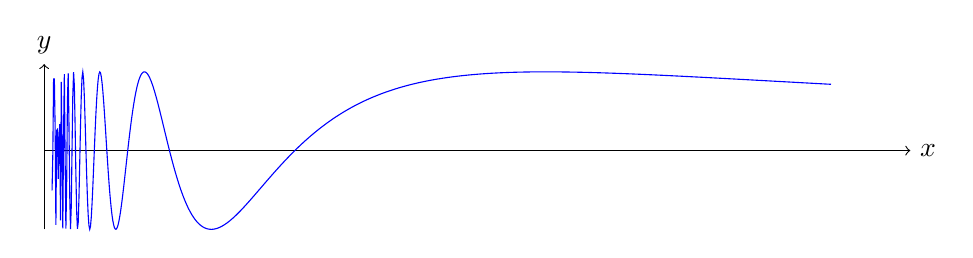
\begin{tikzpicture}[x=10cm]
        \draw[->] (0,0) -- (1.1,0) node[right] {$x$};
        \draw[->] (0,-1) -- (0,1.1) node[above] {$y$};
        \draw[blue,domain=0.01:1,samples=1000] plot (\x, {sin((1/\x)r)});
\end{tikzpicture}
\end{center}}
\author{Xiang Gao}

\begin{document}
\maketitle

\thispagestyle{empty}
\section*{Introduction}

\lettrine[findent=2pt]{\textbf{O}}{ }h Boy! Topology! The one class that absolutely kicked my ass. If you happened to come across this ``glossary" and only know the word ``Topology" from the ``coffee cup is a doughnuts" joke. Well, I have bad news and good news for ya:
\begin{enumerate}
    \item[B).] You won't see and ``coffee cups" or ``doughnuts" for quite some time;
    \item[G).] But you are going to enjoy all the materials nonetheless, and you'll love ``doughnut" as an object for the rest of your life, spoiler alert: it's called a $2$-D Torus. 
\end{enumerate}

Truth is, you need to have some Analysis background with proofs experience, and remember, you best friend and worst enemy $\dfrac{1}{n}$.

My thought of topologists only caring about ``coffee cups" or ``doughnuts" caused me to name the ``Table of Contents" as ``Clay Mathematics" as you can see on the top of each and every single page, which is a quick link to go back, as well as the bottom right. Note: I was not aware of the Clay Mathematics Institution at all when I began to make this ``glossary", it was a happy coincidence.

So what do topologists actually do? Well...
\begin{center}
    Main goal of topology: Classify topological spaces up to \h.
\end{center}

But that is way too hard! So...

\begin{center}
    More realistic goal: Given topological spaces $X$ and $Y$, decide whether or not they are \hc.
\end{center}

Also note that: topologists are sometimes savages. So $\subset$ means ``subset" or ``inclusion" where as $	\subsetneq$ means ``proper subset" or ``proper inclusion". They also denote collection of set using script letter, like $\mathcal{P}\text{(The power set)}, \mathcal{B}\text{(The set of basis)}, \dots$

Anyway! So what's this ``glossary" actually about? Well, when I was busying getting my life totally destroyed by Topology, I found this way to be a really neat way for me to learn harder mathematical concept, and since I will go to graduate school for mathematics one day, it only makes sense for me keep on adding more and more to this document as well as the following:
\begin{enumerate}
    \item[1.] \href{https://www.overleaf.com/project/616b3a6756e3c97b342c6a36}{On-Going Analysis}
    \item[2.] \href{https://www.overleaf.com/project/61843474f70cad11d2caf20f}{Never-Ending Algebra}
\end{enumerate}

The creation of this document involves but not limited to 
\begin{enumerate}
    \item[1.] \emph{Topology} by James Munkers;
    \item[2.] \emph{Counterexamples in Topology} by Lynn Arthur Steen.
\end{enumerate}

And here's the most sincere thanks for all the support and encouragement I got when I was so beaten down by Topology and this Glossary wouldn't be made without you all: Dr. Matt Young, Jan-Luca, Jasper Swensen, Jessica Jorgensen, Hyrum Hansen, Dr. Micheal Shutlz, Dr. Justin Heavilin, and Dr. David Euler Brown.

\vfill

\begin{minipage}[b]{0.9\textwidth}
\footnotesize\raggedright
\setlength{\parskip}{0.5\baselineskip}
Copyright \copyright \, \the\year{} Xiang Gao\par
\end{minipage}
\vspace*{2\baselineskip}

{\protect\hypertarget{toc}{}}
\tableofcontents

\newpage 
\addcontentsline{toc}{part}{Part 1. Introduction to Topology}
\phantomsection
\addcontentsline{toc}{chapter}{Chapter 1. Topology, MATH 5510}

\phantomsection
\section*{1. Reminders on Continuity}
\addcontentsline{toc}{section}{1. Reminders on Continuity}
\phantomsection
\subsection*{1. Continuity}
\addcontentsline{toc}{subsection}{1. Continuity}
\begin{customdefinition}{1.1}[Continuous Function form $\mathbb{R} \longrightarrow \mathbb{R}$]\hypertarget{d_1.1}{\hyperlink{d_3.1}{Click here if you want to know another definition}}
\begin{enumerate}
    \item[1).] A function $f: \mathbb{R} \longrightarrow \mathbb{R}$ is continuous at a point $x \in \mathbb{R}$, if, for all $\epsilon > 0$, there exists a $\delta$ such that 
    $$\left|f(x) - f(y)\right| < \epsilon\,\,\, \text{ whenever }\,\,\, |x- y| < \delta$$
    \item[2).] A function $f: \mathbb{R} \longrightarrow \mathbb{R}$ is continuous if it is continuous at every point $x\in \mathbb{R}$.
\end{enumerate}
\end{customdefinition}

\begin{customdefinition}{1.2}[Euclidean Distance]
Recall that the (Euclidean) distance between two points
$$x = (x_1, \dots, x_n),\,\,\,\,y = (y_1, \dots, y_n)$$
in $\mathbb{R}^n$ is 
$$||x - y|| = \sqrt{(x_1 - y_1)^2 + \dots + (x_n - y_n)^2}$$
\end{customdefinition}

\begin{customdefinition}{1.3}[Continuous Function form $\mathbb{R}^n \longrightarrow \mathbb{R}^m$](So far still good? Well, check this out!)
\begin{enumerate}
    \item[1).] A function $f: \mathbb{R}^n \longrightarrow \mathbb{R}^m$ is continuous at a point $x \in \mathbb{R}^n$, if, for all $\epsilon > 0$, there exists a $\delta > 0$ such that 
    $$\lvert\lvert f(x) - f(y)\rvert\rvert < \epsilon\,\,\, \text{ whenever }\,\,\, \lvert\lvert x - y \rvert\rvert < \delta$$
    \item[2).] A function $f: \mathbb{R}^n \longrightarrow \mathbb{R}^m$ is continuous if it is continuous at every point $x\in \mathbb{R}^n$.
\end{enumerate}
\end{customdefinition}

\begin{customdefinition}{1.4}[Open Ball]
Let $x \in \mathbb{R}^n$ and $\delta > 0$. The open ball at radius $\delta$ centered at x is the set
$$B_\delta (x) = \left\{y \in \mathbb{R}^n \Big| \lvert\lvert x - y\rvert\rvert < \delta\right\}$$
\end{customdefinition}

\begin{customdefinition}{1.5}[Continuity (Reformulated)]
A function $f: \mathbb{R}^n \longrightarrow \mathbb{R}^m$ is continuous at a point $x \in \mathbb{R}^n$, if, for all $\epsilon > 0$, there exists a $\delta > 0$ such that 
    $$f(y) \in B_\epsilon (f(x)) \text{ whenever } y \in B_\delta (x)$$
That is the same as 
    $$f(B_\delta (x)) \subset B_\epsilon (f(x))$$
In words, $f$ is continuous at $x\in \mathbb{R}^n$ if for any $\epsilon > 0$, there exists a $\delta > 0$ such that $f$ sends to open ball of radius $\delta$ at $x$ into the open ball at radius $\epsilon$ at f(x). This sentence gives a precise definition of ``$f$ preserves closeness".\\
In my own words, the image of the open ball of $x$ has to be a subset of the open ball centered at the image of $x$.
\end{customdefinition}

\begin{customdefinition}{1.6}[Open Sets] (Oooohhhhhh! Boy! Here we go!!!!)\\
A subset $U\subset \mathbb{R}^n$ is called open if for all $u \in U$, there exist an $r>0$ such that $$B_r(u) \subset U$$
Open sets, in their generalized form, are fundamental objects in topology.
\end{customdefinition}

\begin{customdefinition}{1.7}[Pre-image] If $f: X \longrightarrow Y$ is a function between sets and $U \subset Y$ is a subset, its pre-image is 
$$f^{-1}(U) = \left\{x\in X \Big| f(x) \in U\right\}$$
\end{customdefinition}

\begin{customthm}{1.1}
A function $f: \mathbb{R}^n \longrightarrow \mathbb{R}^m$ is continuous if and only if, for any open set $U \subset \mathbb{R}^m$, the set $f^{-1}(u) \subset \mathbb{R}^n$ is open.
\end{customthm}

\begin{proof}
First assume that $f$ is continuous and let $U \subset \mathbb{R}^m$ be open. We need to show that $f^{-1}(u) \subset \mathbb{R}^n$ is open. So, let $x \in f^{-1}(u)$, that is 
$$f(x) \in U$$
Since $U$ is open, there exists an $\epsilon > 0$ such that 
$$B_\epsilon(f(x)) \subset U$$
Since $f$ is continuous, there exists a $\delta > 0$ such that 
$$f(B_\delta(x))\subset B_\epsilon(f(x)) \subset U$$
This implies that 
$$B_\delta (x) \subset f^{-1}(U),$$
proving that $f^{-1}(u)$ is open.\\
To prove the converse, suppose that if $U \subset \mathbb{R}^m$ is open, then so too if $f^{-1} (u)$. Let $x \in \mathbb{R}^n$ and $\epsilon > 0$ be given. Then $B_\epsilon(f(x)) \subset \mathbb{R}^m$ is open, so that
$$f^{-1}\left(B_\epsilon(f(x))\right) \subset \mathbb{R}^n$$
is open. Note that $x\in f^{-1}\left(B_\epsilon(f(x))\right)$. So there exists a $\delta > 0$ such that 
$$B_\delta(x) \subset f^{-1} (B_\epsilon (f(x)))$$
that is
$$f(B_\delta(x)) \subset B_\epsilon(f(x))$$
This proves that $f$ is continuous at $x\in\mathbb{R}^n$. Since $x$ was arbitrary, $f$ is continuous.
\end{proof}

\begin{customdefinition}{1.8}[Closed Sets] A subset $A \subset \mathbb{R}^n$ is called closed if its complement
$$A^c = \mathbb{R}^n \setminus A =\left\{x \in \mathbb{R}^n \mid x \notin A\right\}$$
is an open subset.\\
$A$ is closed $\iff$ for each $u\notin A$, there exists an open ball $B_r(u)$ which does not intersect $A$.
\end{customdefinition}

       
\newpage
\phantomsection
\section*{2. Topological Spaces}
\addcontentsline{toc}{section}{2. Topological Spaces}
\phantomsection
\subsection*{1. Topology}
\addcontentsline{toc}{subsection}{1. Topology}
\begin{customdefinition}{2.1}[Topology](Here's where everything starts to go south...)
\begin{enumerate}
    \item[1). ] Let $X$ be a set. A topology on $X$ is a set $\tau$ of subsets of $X$, called open sets, such that 
        \begin{enumerate}
            \item[i).] $\varnothing, \,\,X$ are open sets
            \item[ii).] If $\left\{U_i\right\}_{i \in I}$ is an arbitrary collection of open sets, then $\underaccent{i \in I}{\bigcup}U_i$ is open
            \item[iii).] If $\left\{U_i\right\}_{i \in I}$ is a finite collection of open sets, then $\underaccent{i \in I}{\bigcap}U_i$ is open
        \end{enumerate}
    \item[2). ]A topological space is a set $X$ with a chosen topology $\tau$.\\
            For example, the Euclidean topology on $\R^n$,  $\tau_{\text{Euclidean}} = \left\{U \subset \R^n \mid U \text{open in the sense of Definition 1.6}\right\}$
\end{enumerate}
\end{customdefinition}

\begin{customdefinition}{2.2}[Discrete Topology]
Let $X$ be a set. The discrete topology on $X$ is 
    $$\tau_{\text{dis}} = \left\{U \subset X\right\}$$
    That is, every subset of $X$ is open. It is immediate that $\tau_{\text{dis}}$ is indeed a topology.\\
Book: If $X$ is any set, the collection of all subsets of $X$ is a topology on $X$, it is called discrete topology.
\end{customdefinition}

\begin{customdefinition}{2.3}[Indiscrete(trivial) Topology]
Let $X$ be a set. The indiscrete(trivial) topology on $X$ is 
    $$\tau_{\text{ind}} = \left\{\varnothing, X\right\}$$
    That is, every subset of $X$ is open. It is immediate that $\tau_{\text{dis}}$ is indeed a topology.\\
The indiscrete topology is very ``small" in the sense that all points of $X$ are clumped together! On the other hand, the discrete topology is very ``large" (Spoiler Alert: is it Hausdorff?).\\
Book: The collection of consisting of $X$ and $\varnothing$ only is a topology on $X$, we shall call it the indiscrete topology.
\end{customdefinition}

\begin{customdefinition}{2.4}[The Finite Complement Topology]
Let $X$ be a set. The finite Complement topology on $X$ is 
    $$\tau_{\text{fin}} = \left\{U\subset X \mid X \setminus U \text{ is a finite set or is } X \right\}$$
    That is, every subset of $X$ is open. It is immediate that $\tau_{\text{dis}}$ is indeed a topology.\\
Book: Let $X$ be a set; let $\tau_f$ be the collection of all subsets $U$ of $X$ such that $X-U$ either is finite or is all of $X$. Then $\tau_f$ is a topology on $X$, called the finite complement topology. 
\end{customdefinition}
\begin{proof}
Check that $2.4$ is a topology
\begin{enumerate}
    \item[1).] $\varnothing \in \tau_f$ since $X\setminus X$ is finite. $X\in \tau_f$ since $X\setminus\varnothing$ is all of $X$.
    \item[2).] Say $\left\{U_i\right\}_{i\in I}$ are open, i.e.
               $$X \setminus U_i \text{ is finite on } X$$
               then
               $$X \setminus \underaccent{i \in I}{\bigcup}U_i = \underaccent{i \in I}{\bigcap}\left(X \setminus U_i\right)$$
               is the intersection of finite sets, so is itself finite. Hence, $\underaccent{i \in I}{\bigcup}U_i$ is open.
    \item[3).] Say $\left\{U_i\right\}_{i\in I}$ is a finite collection of open sets. Then
               $$X \setminus \underaccent{i \in I}{\bigcap}U_i = \underaccent{i \in I}{\bigcup}\left(X \setminus U_i\right)$$
               is a finite union of finite sets and so is itself finite. Hence, $\underaccent{i \in I}{\bigcap}U_i$ is open.          
\end{enumerate}
Therefore, $\tau_f$ is a topology.
\end{proof}

\begin{customdefinition}{2.5}[Coarser and Finer]
Let $X$ be a set with topologies $\tau$ and $\tau'$. We call $\tau$ coarser than $\tau \subset \tau'$. In this situation, we call $\tau'$ finer than $\tau$. If either $\tau \subset \tau'$ or $\tau' \subset \tau$, then we call $\tau$ and $\tau'$ comparable.
\end{customdefinition}

\newpage

\phantomsection
\subsection*{2. Basis for Topology}
\addcontentsline{toc}{subsection}{2. Basis for Topology}

\begin{customdefinition}{2.6}[Basis for a Topology]
Let $X$ be a set. A basis for a topology on $X$ is a collection $\B$ of subsets of $X$ such that
\begin{enumerate}
    \item[1).] Every $x \in X$ is contained in some $B \in \B$
    \item[2).] If $x\in X$ with $B_1, B_2 \in \B$ containing $x$ then there exists $B_3 \in \B$ such that 
                $$x\in B_3 \subset B_1 \cap B_2$$
                In pictures:
                \begin{center}
                \begin{tikzpicture}
                \draw[red, semitransparent, dashed, thick] (-1.5,0) circle[radius=66pt];
                \node[label, red] at (-1.6,1) {$B_1$};
                \draw[red, semitransparent, dashed, thick] (1.5,-1) circle[radius=88pt];
                \node[label, red] at (1.5,-1) {$B_2$};
                \draw[red, semitransparent, dashed, thick] (-0.3,-0.3) circle[radius=24pt];
                \node[label, blue] at (-0.3,-0.3) {$x$};
                \node[label, red] at (0,0) {$B_3$};
                \end{tikzpicture}
                \end{center}
    \end{enumerate} 
\end{customdefinition}


\begin{customthm}{2.1}
Let $\B$ be a basis for a topology on $X$. Then 
$$\tau = \left\{U \subset X \mid \text{ for all $u \in U$, there exists a $B \in \B$ such that $u \in B \subset U$}\right\}$$
is a topology on $X$.
\end{customthm}

\begin{customdefinition}{2.6}
The topology $\tau$ of Theorem $2.1$ is called the topology generated by $\B$.\\
Book: A subset $U$ of $X$ is said to be open in $X$ (that is, to be an element of $\tau$) if for each $x\in U$, there is a basis element $B \in \B$ such that $x \in B$ and $B \subset U$. Note that each basis element is itself an element of $\tau$.
\end{customdefinition}

\begin{customlemma}{2.2}
Let $\B$ be a basis for a topology $\tau$ on a set $X$. Then $U \subset X$ is open (i.e. $U\in \tau$) if and only if $U$ is a union of elements of $\B$.
\end{customlemma}

\begin{proof}
Given a collection of elements of $\B$, they are also elements in $\tau$. Because $\tau$ is a topology, their union is in $\tau$. Conversely, given $U \in \tau$, choose for each $x\in U$ an element $B_x$ of $\B$ such that $x \in B_x \subset U$. Then $U = \underaccent{x \in U}{\bigcup} B_x$, so $U$ equals a union of elements of $\B$. 
\end{proof}

\begin{customlemma}{2.3}
Let $(X, \tau)$ be a topological space. Let $\mathcal{C}$ be a collection of open sets such that for each open set $U$ and $x \in U$, there exists a $C\in \mathcal{C}$ such that $x \in C \subset U$. Then $\mathcal{C}$ is a basis for $\tau$.
\end{customlemma}

\begin{proof}
We need to show two things:
\begin{enumerate}
    \item[1).] $\mathcal{C}$ is a basis for a topology on $X$.\\
            The first condition for a basis is easy: Given $x\in X$, since $X$ is itself an open set, there is by hypothesis an element $C$ of $\mathcal{C}$ such that $x\in C \subset X$. To check the second condition, let $x$ belong $C_1 \cap C_2$, where $C_1$ and $C_2$ are elements of $\mathcal{C}$. Since $C_1$ and $C_2$ are open, so is $C_1 \cap C_2$. Therefore, there exists by hypothesis an element $C_3$ in $\mathcal{C}$ such that $x \in C_3 \subset C_1 \cap C_2$.
    \item[2).] The topology $\tau_{\mathcal{C}}$ generated by $\mathcal{C}$ is $\tau$.\\
            Let $U \subset X$ be open. For each $u \in U$, there exists a $C_u \in \mathcal{C}$ with $u \in C_u \subset U$. Then 
                    $$U = \underaccent{u \in U}{\bigcup} C_u$$
            By Lemma $2.2$, the right hand side is in $\tau_{\mathcal{C}}$, that is $\tau \subset \tau_{\mathcal{C}}$. Since $\mathcal{C} \subset \tau$, again by Lemma $2.2$, we have $\tau_{\mathcal{C}} \subset \tau$. So, $\tau = \tau_{\mathcal{C}}$.
\end{enumerate}
\end{proof}

\newpage

\begin{customdefinition}{2.7}
A subbasis $\mathcal{S}$ for a topology on $X$ is a collection of subsets of $X$ whose union is equal to $X$:
    $$\underaccent{S \in \mathcal{S}}{\bigcup}S = X$$
\end{customdefinition}

\begin{customlemma}{2.4}
Let $\mathcal{S}$ be a subbasis for a topology on $X$. Then 
$$\tau_{\mathcal{S}} = \left\{U \subset X \mid \text{ $U$ is a union of finite intersections of elements of $\mathcal{S}$}\right\}$$
is a topology on $X$.
\end{customlemma}

\phantomsection
\subsection*{3. Product Topology}
\addcontentsline{toc}{subsection}{3. Product Topology}

\begin{customdefinition}{2.8}[Product Topology]
Let $X, Y$ be topological spaces. The product topology on 
$$X \times Y = \left\{(x,y) \mid x\in X, y\in Y\right\}$$
is the topology generated by the basis 
$$\B = \left\{u \times v \mid u \subset X \text{ is open, } v\subset Y \text{ is open}\right\}$$
\end{customdefinition}

\begin{proof}
Check that $\B$ is indeed a basis for a topology on $X\times Y$.
\begin{enumerate}
    \item[1).] $\B$ covers $X \times Y$: Let $(x, y) \in X \times Y$. Since $X \subset X$ and $Y \subset Y$ are open, $X \times Y \in \B$ and $\B$ covers. Or, it's already trivial, since $X \times Y$ is itself a basis element.
    \item[2).] Say $u \times v, \,\, u' \times v' \in \B$ and 
                $$(x, y) \in (u\times v) \cap (u' \times v') = (u \cap u') \times (v \cap v')$$
                Since $u \cap u',\,\, v \cap v'$ are open, we have
                $$(u\times v) \cap (u' \times v') \in \B$$
\end{enumerate} 
\end{proof}

\begin{customthm}{2.5}
Let $X$ and $Y$ be topological spaces with bases $\B$ and $\mathcal{C}$, respectively, then 
    $$\mathcal{D} = \left\{u\times v\mid u\in \B, v \in \mathcal{C}\right\}$$
    is a basis for the product topology on $X \times Y$.
\end{customthm}

\begin{proof}
We will use Lemma $2.3$. So, let $W \subset X \times Y$ be open and $(x,y) \in W$. By the definition of the product topology,
$$W = \underaccent{i}{\bigcup} u_i \times v_i$$
for some $u_i \in \B$ and $v_i \in \mathcal{C}$. Then 
$$(x, y) \in \underbrace{u_j \times v_j}_{in \,\mathcal{D}} \subset W$$
for some $j$. By Lemma $2.3$, we are done.
\end{proof}

\begin{customdefinition}{2.9}[Projections]
Let $\pi_x: X \times Y \longrightarrow X$ be defined by the equation:
$$\pi_x(x,y) = x$$
Let $\pi_y: X \times Y \longrightarrow Y$ be defined by the equation:
$$\pi_y(x,y) = y$$
The maps $\pi_x$ and $\pi_y$ are called the projections of $X \times Y$ onto (surjective) its its first and second factors, respectively. Given any subset $U \subset X$ is open, we have
$$\pi_x^{-1}(U) = \left\{(x, y) \in X\times Y \mid x\in U\right\}$$
In particular, if $X$ and $Y$ are topological spaces and $U\subset X$ is open, then so too is $\pi_x^{-1}(U)$.
\end{customdefinition}

\begin{customthm}{2.6}
Let $X, Y$ be topological spaces. Then 
$$\mathcal{S} = \left\{\pi_x^{-1}(U) \mid U\subset X \text{ is open}\right\} \cup \left\{\pi_y^{-1}(U) \mid V\subset Y \text{ is open}\right\}$$
is a subbasis for the product topology on $X \times Y$.
\end{customthm}

\newpage

\begin{proof}
Let $\tau$ be the product topology on $X \times Y$ and $\tau_{\mathcal{S}}$ the topology generated by $\mathcal{S}$. It is immediate that $\tau_{\mathcal{S}} \subset \tau$. To see that $\tau \subset \tau_{\mathcal{S}}$, note that if $U \subset X$ and $V \subset Y$ are open, then 
$$\pi_x^{-1}(U) \cap \pi_y^{-1}(V) = U \times V \in \tau_{\mathcal{S}}$$
Since $\left\{U \times V \mid U \subset X \text{ open, } V \subset Y \text{ open}\right\}$ is a basis for $\tau$, we get $\tau \subset \tau_{\mathcal{S}}$.
\end{proof}

\phantomsection
\subsection*{4. Subspace Topology}
\addcontentsline{toc}{subsection}{4. Subspace Topology}

\begin{customdefinition}{2.10}[Subspace Topology]
Let $(X, \tau)$ be a topological space and $Y \subset X$ a subset. Then 
$$\tau_Y = \left\{Y \cap U \mid U \subset X \text{ is open}\right\}$$
is the subspace topology on $Y$. With this topology, $Y$ is called a subspace of $X$; its open sets consist of all intersections of opens sets of $X$ and $Y$.
\end{customdefinition}

\begin{customlemma}{2.7}
The subspace topology $\tau_Y$ is a topology.
\end{customlemma}
\begin{proof}
We have
\begin{align*}
    \varnothing &= Y \cap \varnothing \in \tau_Y\\
    Y & = Y \cap X \in \tau_Y
\end{align*}
Let $\left\{U_i\right\}_{i \in I}$ be open in $Y$ (so $U_i \in \tau_Y$). Then 
$$U_i = Y\cap V_i$$
for some $V_i \subset X$ open and 
\begin{align*}
  \underaccent{i\in I}{\bigcup} U_i &= Y \cap \underbrace{\left(\underaccent{i\in I}{\bigcup} V_i\right)}_{\text{open in $X$}} \in \tau_Y \\
  \underaccent{i\in I}{\bigcap} U_i &= Y \cap \overbrace{\left(\underaccent{i\in I}{\bigcap} V_i\right)}_{} \in \tau_Y
\end{align*}
if $|I| < \infty$.
\end{proof}

\begin{customlemma}{2.8}
Let $Y \subset X$ be a subspace. If $U \subset Y$ is open and $Y \subset U$ is open, then $U \subset X$ is open.
\end{customlemma}

\begin{proof}
Since $U$ is open in $Y$, $U = Y \cap V$ for some set $V$ open in $X$. Since $Y$ and $V$ are both open in $X$, so is $Y \cap V$.
\end{proof}

\begin{customlemma}{2.9}
Let $X$ be a topological space with basis $\B$ and $Y\subset X$ a subset. Then
$$\B_Y = \left\{Y\cap B \mid B \in \B\right\}$$
is a basis for the subspace topology of $Y$. In words, a basis for $X$ induces a basis for the subspace $Y \subset X$.
\end{customlemma}

\begin{proof}
Given $U$ is open in $X$ and given $y \in U \cap Y$, we can choose an element $B$ of $\B$ such that $y \in B \subset U$. Then $y \in B \cap Y \subset U \cap Y$. It follows from Lemma $2.3$ that $\B_Y$ is a basis for the subspace topology on $Y$.
\end{proof}

\begin{customthm}{2.10}
Let $X, Y$ be topological spaces with subsets $A\subset X$ and $B \subset Y$. Then the subspace topology on $A\times B \subset X \times Y$ is the same as the product topology on $A \times B$.
\end{customthm}

\begin{proof}
A basis element of the product topology on $X \times Y$ is $U\times V$, where $U\subset X$ and $V \subset Y$ are open. Then 
$$\left(A \times B\right) \cap \left(U \times V\right) = \left(A\cap U\right) \times \left(B \cap V\right)$$
is a basis element for the subspace topology on $A \times B$. But the RHS is a basis element for the product topology on $A\times B$.
\end{proof}

\begin{customdefinition}{2.11}
Let $X$ be a topological space. A subset $A \subset X$ is called closed if $A^c = X \setminus A \subset X$ is open.
\end{customdefinition}

\begin{customthm}{2.11}
Let $X$ be a topological space
\begin{enumerate}
    \item[1).] $\varnothing$ and $X$ are closed.
    \item[2).] Arbitrary intersections of closed sets are closed:\\
                If $\left\{A_i\right\}_{i \in I}$ is a collection of closed sets, then $\underaccent{i\in I}{\bigcap} A_i$ is closed.
    \item[3).] Finite unions of closed sets are closed:\\
                If $\left\{A_i\right\}_{i \in I}$ is a finite collection of closed sets, then $\underaccent{i\in I}{\bigcup} A_i$ is closed.
\end{enumerate}
\end{customthm}

\newpage

\begin{proof}
\begin{enumerate}
    \item[1).] $\varnothing$ and $X$ are closed because they are the complements of the open sets $X$ and $\varnothing$, respectively.
    \item[2).] Given a collection of closed sets $\left\{A_i\right\}_{i \in I}$, we apply DeMorgan's Law,
        $$X - \underaccent{i \in I}{\bigcap} A_i = \underaccent{i\in I}{\bigcup} \left(X - A_i\right)$$
        Since the sets $X - A_i$ are open by definition, the right side of this equation represents an arbitrary union of open sets, and is thus open. Therefore, $\underaccent{i \in I}{\bigcap} A_i$ is closed.
    \item[3).] Similarly, if $A_i$ is closed for $i = 1, 2, \dots, n \in I $, consider the equation
        $$X - \underaccent{i \in I}{\bigcup} A_i = \underaccent{i\in I}{\bigcap} \left(X - A_i\right)$$
        The set on the right hand side is a finite intersection of open sets and is therefore open. Hence $\underaccent{i \in I}{\bigcup} A_i$ is closed.
\end{enumerate}
\end{proof}

\begin{customlemma}{2.12}
Let $Y \subset X$ be a subspace and $A \subset Y$ a subset. Then $A\subset Y$ is closed if and only if $A = Y \cap C$ for a closed set $C \subset X$. 
\end{customlemma}

\begin{proof} If and only if...
\begin{enumerate}
    \item[1).]Assume $A\subset Y$ is closed. Then $Y \setminus A$ is open so that $Y \setminus A = Y \cap U$ for an open $U \subset X$. Then
    \begin{align*}
        A & = Y \setminus\left(Y\setminus A\right)\\
          & = Y \setminus\left(Y \cap U\right)\\
          & = Y \cap \left(X \setminus U\right)
    \end{align*}
    The set $X \setminus U$ is closed in $X$, so we can take $C = X \setminus U$.
    \item[2).]Conversely, assume that $A = Y\cap C$ for $C \subset X$ closed. Then, by the above, we see that
    $$Y \setminus A = Y \cap \left(X \setminus C\right)$$
    The set $X \setminus C$ is open in $X$, so that $Y \setminus A$ is open in $Y$. Therefore, $A \subset Y$ is closed.
\end{enumerate}
\end{proof}

\phantomsection
\subsection*{5. Interior and Closure}
\addcontentsline{toc}{subsection}{5. Interior and Closure}

\begin{customdefinition}{2.12}[Interior and Closure]
Let $X$ be a topological space and $Y \subset X$ a subset.
\begin{enumerate}
    \item[1).] The interior of $Y (\text{in }X)$ is the union of all open sets contained in $Y$, and is denoted by $Int(Y)$.
    \item[2).] The closure of $Y (\text{in }X)$ is the intersection of all closed sets of $X$ which contain $Y$, and is denoted by $\overline{Y}$.
\end{enumerate}
$$Int(Y) \subset Y \subset \overline{Y}$$
If $Y$ is open, $Y = Int(Y)$; while if $Y$ is closed, $Y = \overline{Y}$
\end{customdefinition}

\begin{customlemma}{2.13}
Let $X$ be a topological space and $Y \subset X$ a subset. Then $Int(Y) \subset X$ is open and $\overline{Y} \subset X$ is closed.
\end{customlemma}

\begin{customlemma}{2.14}
Let $X$ be a topological space and $Y \subset X$ a subset.
\begin{enumerate}
    \item[1).] $Y$ is open if and only if $Int(Y) = Y$
    \item[2).] $Y$ is closed if and only if $Y = \overline{Y}$
\end{enumerate}
\end{customlemma}

\begin{customthm}{2.15}
Let $X$ be a topological space with a subset $Y$.
\begin{enumerate}
    \item[1).] Then $x \in \overline{Y}$ if and only if any open set $x\in U \subset X$ intersects $Y$.
    \item[2).] Let $\B$ be a basis for the topology on $X$. Then $x \in \overline{Y}$ if and only if every $B \in \B$ with $x \in B$ intersects $Y$.
\end{enumerate}
\end{customthm}

\begin{customdefinition}{2.13}[Limit Points]
Let $X$ be a topological space and $Y \subset X$ a subset. A point $l \in X$ is called a limit point of $Y$ (or cluster/accumulation point) if every open set $U \subset X$ which contains $l$ intersects $Y$ at a point different from $l$. Said differently, $l$ is a limit point of $A$ if it belongs to the closure of $A - \left\{x\right\}$. The point $l$ may lie in $A$ or not; for this definition it does not matter.
\end{customdefinition}

\begin{customthm}{2.16}
Let $X$ be a topological space with a subset $Y \subset X$. Then
$$\overline{Y} = Y \cup \left\{\text{limit points of Y}\right\} = Y \cup Y'. \,\,\,\,\,\,\, (Y' := \left\{\text{limit points of Y}\right\})$$
\end{customthm}

\begin{proof}
Let $l$ be a limit point of $Y$. Then every open set containing $l$ intersects $Y$. By Theorem $2.15$, $x\in \overline{Y}$. Hence, $\overline{Y} \supset Y \cup Y'$. For the reverse inclusion, let $x \in \overline{Y}$. Say $x \notin Y$; we prove that $x\in Y'$. Again by Theorem $2.15$, any open set $x \in U \subset X$ intersects $Y$. Since $x\notin Y$, we see that any open set containing $x$ intersects $Y$ at a point different from $l$. So, $x \in Y'$.
\end{proof}

\begin{customcoro}{2.17}
A subset $Y \subset X$ is closed if and only if it contains all of its limit points.
\end{customcoro}

\begin{customdefinition}{2.13}[Boundary]
Let $X$ be a topological space. The \emph{boundary} of a subset $A \subset X$ is defined to be
$$\partial A = \overline{A} \cap \overline{X \setminus A},$$
where $\overline{(-)}$ denotes closure.
\end{customdefinition}

\phantomsection
\subsection*{6. Hausdorff Spaces}
\addcontentsline{toc}{subsection}{6. Hausdorff Spaces}

\begin{customdefinition}{2.14}[Hausdorff Spaces]
A topological space $X$ is called Hausdorff if for every pair of distinct points $x, x' \in X$, there exists open sets 
$$x \in U \subset X,\,\,\,\,\,\,\, x' \in U' \subset X$$
such that $U \cap U' = \varnothing$\\
In pictures:
    \begin{center}
    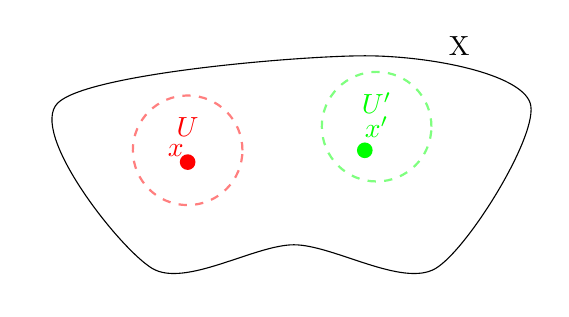
\begin{tikzpicture}[scale = 0.3]
    \draw[red, semitransparent, dashed, thick] (-4.5,-2) circle[radius=66pt];
    \node[label, red] at (-4.5,-1) {$U$};
    \node[label, red] at (-5,-2) {$x$};
    \node[circle, fill, red, inner sep=2pt] at (-4.5, -2.5) {};
    \draw[green, semitransparent, dashed, thick] (3.5,-1) circle[radius=66pt];
    \node[label, green] at (3.5,0) {$U'$};
    \node[label, green] at (3.5,-1) {$x'$};
    \node[circle, fill, green, inner sep=2pt] at (3, -2) {};
    \draw plot [smooth cycle] coordinates {(0,-6) (-6,-7) (-10,0) (3,2) (10,0) (6,-7) } node at (7,2.4) {X};
    \end{tikzpicture}
    \end{center}
\end{customdefinition}

\begin{customthm}{2.18}
Let $X$ be a Hausdorff (topological) space. Then any finite subset $A \subset X$ is closed. In particular, points are closed in $X$. 
\end{customthm}

\begin{customdefinition}{2.15}
Let $X$ be a topological space. A sequences of points $\left\{x_n\right\}_{n \geqslant 1}$ in $X$ converges to $x \in X$ if for any open set $x \in U \subset X$, there exists an $N > 0$ such that $x_n \in U$ whenever $n>N$.
\end{customdefinition}

\begin{customthm}{2.19}
Let $X$ be a Hausdorff space. A sequence in $\left\{x_n\right\}_{n \geqslant 1}$ in $X$ converges to at most one point of $X$; if it exists, this point is called the limit of $\left\{x_n\right\}$ and denoted by $\displaystyle\lim_{n \to \infty} x_n$.
\end{customthm}

\begin{proof}
Suppose that $\left\{x_n\right\}_{n \geqslant 1}$ converges to distinct points $a, b \in X$. Since $X$ is Hausdorff, there exists open set 
$$a \in U \subset X, \,\,\,\, b \in V \subset X$$
such that $U \cap V = \varnothing$. Since $\left\{x_n\right\}_{n \geqslant 1}$ converges to $a$, there exists $N > 0$ such that $x_n \in U$ if $n>N$. Similarly, there exists an $M>0$ such that $x_n \in V$ if $n>M$. Let $L = max\left\{M,N\right\}$. Then $x_n \in U\cap V$ if $n > L$. But $U\cap V = \varnothing$, a contradiction.
\end{proof}

\begin{customthm}{2.20}[Fantastic Top-spaces and Where to Find Them](Hausdorff)
\begin{enumerate}
    \item[1).] Let $X, Y$ be Hausdorff spaces. Then $X \times Y$ is Hausdorff.
    \item[2).] Let $X$ be a Hausdorff space and $Y \subset X$ a subset. Then $Y$, with the subspace topology, is Hausdorff.
\end{enumerate}
\end{customthm}

\begin{proof}
\begin{enumerate}
    \item[1).]Let $(x, y), (x', y') \in X\times Y$ be distinct. Suppose that $x \neq x'$. Since $X$ is Hausdorff, there exist open sets 
    $$x \in U \subset X, \,\,\,\,\,\, x' \in U' \subset X$$
    such that $U\cap U' = \varnothing$. Then 
    $$(x, y) \in U \times Y, \,\,\,\,\,\, (x', y') \in U' \times Y$$
    are disjoint open sets. If $x = x'$, then $y = y'$ and we can modify the previous argument.
    \item[2).]Let $y, y'\in Y$ be distinct. Since $X$ is Hausdorff, there exist open sets $y \in U \subset X, \,\, y' \in U' \subset X$ such that $U\cap U' = \varnothing$. Then $y \in U \cap Y \subset Y,\,\, y' \in U' \cap Y \subset Y$ are open sets in $Y$ such that 
    $$\left(U \cap Y \right) \cap \left(U' \cap Y \right) = \left(U \cap U' \right)\cap Y = \varnothing$$
    So, $Y$ is Hausdorff.
\end{enumerate}
\end{proof}

\newpage
\phantomsection
\section*{3. Continuous Functions}
\addcontentsline{toc}{section}{3. Continuous Functions}

\phantomsection
\subsection*{1. Continuous Functions}
\addcontentsline{toc}{subsection}{1. Continuous Functions}

\begin{customdefinition}{3.1}[Continuous Functions]\hypertarget{d_3.1}{\hyperlink{d_1.1}{Click here to be more sane.}}\\
Let $X, Y$ be topological space. A continuous function $f: X \longrightarrow Y$ is a function at underlying sets such that, for each open set $U \subset Y$, the preimage 
$$f^{-1}(U) = \left\{x \in X \mid f(x) \in U\right\}$$
is open (in $X$).\\
\emph{To know more about the notation please go to Appendix $1$.}
\end{customdefinition}

\begin{customlemma}{3.1}
Let $\B$ be a basis for the topology on $Y$. A function $f: X \longrightarrow Y$ is continuous if and only if $f^{-1}(\B)$ is open for all $B \in \B$.
\end{customlemma}

\begin{customthm}{3.2}
Let $f: X \longrightarrow Y$ be a function between topological spaces. The following statements are equivalent:
\begin{enumerate}
    \item[1).] f is continuous.
    \item[2).] For any subset $A \subset X$, we have $f(\overline{A}) \subset \overline{f(A)}$.
    \item[3).] For any closed set $C \subset Y$, the preimage $f^{-1}(C) \subset X$ is closed.
    \item[4).] For each $x \in X$ and open set $f(x) \in V \subset Y$, there exists an open set $x \in U \subset X$ such that $f(u) \subset V.$
\end{enumerate}
If the condition in $(4)$ holds for the point $x$ of $X$, we say that $f$ is continuous at the point $x$.
\end{customthm}

\begin{proof}
We show that $(1) \implies (2) \implies (3) \implies (1)$ and $(1) \implies (4) \implies (1)$
\begin{description}
\item[$1) \implies 2)$.] Assume that $f$ is continuous. Let $A$ be a subset of $X$. We show that if $x \in \overline{A}$, then $f(x) \in \overline{f(A)}$. Let $V$ be a neighborhood of $f(x)$ ($V$ is an open set containing $x$). Then $f^{-1}(V)$ is an open set of $X$ containing $x$; it must intersect $A$ in some point $y$. Then $V$ intersects $f(A)$ in the point $f(y)$, so that $f(x) \in \overline{f(A)}$, as desired.
\item[$2) \implies 3)$.] Let $B$ be closed in $Y$ and let $A = f^{-1}(B)$. We wish to prove that $A$ is closed in $X$; we show that $\overline{A} = A$. By elementary set theory, we have $f(A) = f(f^{-1}(B)) \subset B$. Therefore, if $x \in \overline{A}$,
    $$f(x) \in f(\overline{A}) \subset \overline{f(A)} \subset \overline{B} = B,$$
so that $x \in f^{-1}(B) = A$. Thus $\overline{A} \subset A$, so that $\overline{A} = A$, as desired.
\item[$3) \implies 1)$.] Let $V$ be an open set of $Y$. Set $B = Y - V$. Then 
    $$f^{-1}(B) = f^{-1}(Y) - f^{-1}(V) = X - f^{-1}(V)$$
    Now $B$ is a closed set of $Y$. Then $f^{-1}(B)$ is closed in $X$ by hypothesis, so that $f^{-1}(V)$ is open in $X$, as desired.
\item[$1) \implies 4)$.] Let $x \in X$ and let $V$ be a neighborhood of $f(x)$. Then the set $U = f^{-1}(V)$ is a neighborhood of $x$ such that $f(U) \subset V$.
\item[$4) \implies 1)$.] Let $V$ be an open set of $Y$; let $x$ be a point of $f^{-1}(V)$. Then $f(x) \in V$, so that by hypothesis there is a neighborhood $U_x$ of $x$ such that $f\left(U_x\right)\subset V$. Then $U_x \subset f^{-1}(V)$. It follows that $f^{-1}(V)$ can be written as the union of the open sets $U_x$, so that it is open.
\end{description}
\end{proof}

\begin{customthm}{3.3}[Constructing Continuous Functions]
Let $X, Y, Z$ be topological spaces. 
\begin{enumerate}
    \item[a).] (Constant Function) If $f: X \longrightarrow Y$ maps to all of $X$ into the single point $y_0$ of Y, then $f$ is continuous.
    \item[b).] (Inclusion) If $A$ is subspace of $X$, the inclusion function $j: A \longrightarrow X$ is continuous.
    \item[c).] (Composites) If $f: X \longrightarrow Y$ and $g: Y \longrightarrow Z$ are continuous, then the map $g \circ f : X \longrightarrow Z$ is continuous.
    \item[d).] (Restricting the domain) If $f: X \longrightarrow Y$ is continuous, and if $A$ is a subspace of $X$, then the restricted function $f_{\vert A} : A \longrightarrow Y$ is continuous (where $A \subset Y$ is given the subspace topology).
    \item[e).] (Restricting or expanding the range) Let  $f: X \longrightarrow Y$ is continuous. If $Z$ is a subspace of $Y$ containing the image set $f(X)$, then the function $g: X \longrightarrow Z$ obtained by restricting the range of $f$ is continuous. If $Z$ is a space having $Y$ as a subspace, then the function $h: X \longrightarrow Z$ obtained by expanding the range of $f$ is continuous.  
    \item[f).] (Local formulation of continuity) The map $f: X \longrightarrow Y$ is continuous if $X$ can be written as the union of open sets $X = \underaccent{i\in I}{\bigcup}U_{\alpha}$ such that $f_{\vert U_{\alpha}}: U_{\alpha} \longrightarrow Y$ is continuous for each $\alpha$.
\end{enumerate}
\end{customthm}

\newpage

\begin{proof}
Let's proof every single one of them:
\begin{enumerate}
    \item[a).] Let $f(x) =y_0$ for every $x \in X$. Let $V$ be open in $Y$. The set $f^{-1} (V)$ equals $X$ or $\varnothing$, depending on whether $V$ contains $y_0$ or not. In either case, it is open.
    \item[b).] If $U$ is open in $X$, then $j^{-1}(U) = A \cap U$, which is open in $A$ by definition of the subspace topology.
    \item[c).] If $U$ is open in $Z$, then $g^{-1}(U)$ is open in $Y$ and $f^{-1}(g^{-1}(U))$ is open in $X$. But
                $$f^{-1}(g^{-1}(U)) = \left(g \circ f\right)^{-1}(U),$$
                by elementary set theory. (The book really need to drop this ``elementary" notation, makes me feels even dumber.)
    \item[d).] The function $f_{\vert A}$ equals the composite of the inclusion map $j: A \longrightarrow X$ and the map $f: X \longrightarrow Y$, both of which are continuous.
    \item[e).] Let $f: X \longrightarrow Y$ be continuous. If $f(X) \subset Z \subset Y$, we show that the function $g: X \longrightarrow Z$ obtained from $f$ is continuous. Let $B$ open in $Z$. Then $B = Z \cap U$ for some open set $U$ of $Y$. Because $Z$ contains the entire image set $f(X)$,
                $$f^{-1}(U) = f^{-1}(B),$$
                by the elementary set theory (Shut the f**k up!). Since $f^{-1}(U)$ is open, so is $g^{-1}(B)$.\\
                To show $h: X \longrightarrow Z$ is continuous if $Z$ has $Y$ as a subspace, note that $h$ is the composite of the map $f: X \longrightarrow Z$ and the inclusion map $j: Y \longrightarrow Z$.
    \item[f).] By hypothesis, we can write $X$ as a union of open sets $U_{\alpha}$, such that $f_{\vert U_{\alpha}}$ is continuous for each $\alpha$. Let $V$ be an open set in $Y$. Then
                $$f^{-1}(V) \cap U_{\alpha} = \left(f_{\vert U_{\alpha}}\right)^{-1}(V),$$
                because both expressions represent the set of those points $x$ lying in $U_{\alpha}$ for which $f(x) \in V$. Since $f_{\vert U_{\alpha}}$ is continuous, this set is open in $U_{\alpha}$, and hence open in $X$. But
                $$f^{-1}(V) = \underaccent{\alpha}{\bigcup} \left(f^{-1}(V) \cap U_{\alpha}\right),$$
                so that $f^{-1}(V)$ is also open in $X$.
\end{enumerate}
\end{proof}

\begin{customthm}{3.4}[Another Version (Slightly Weaker) of Gluing ($f$ in the previous theorem) For Closed Sets](Ready?)\\
Let $X$ be a topological space with closed subsets $A, B \subset X$ such that $X = A\cup B$. Let 
        $$g: A \longrightarrow Z, \,\,\,\,\, h: B\longrightarrow Z$$
        be continuous functions such that 
        $$g_{\vert A \cap B} = h_{\vert A \cap B}$$
        Then $g$ and $h$ glue to a continuous function 
        \begin{align*}
            f:  X &\longrightarrow Z\\
                x &\longrightarrow \begin{cases}
               g(x), & \text{ if $x\in A$}\\
               h(x), & \text{ if $x\in B$}
               \end{cases}
        \end{align*}
\end{customthm}

\begin{proof}
Recall (Theorem $3.2(3)$) that $f$ is continuous if and only if $f^{-1}(C) \subset X$ is closed for all $C \subset Z$ closed. Basic set theory gives:
    $$f^{-1}(C) = g^{-1}(C) \cap h^{-1}(C).$$
    Since $g, h$ are continuous, $g^{-1}(C) \subset A$ and $h^{-1}(C) \subset B$ are closed. Since $A$ and $B$ are closed in $X$, so too are $g^{-1}(C)$ and $h^{-1}(C)$. Since finite intersections of closed sets are closed, we can conclude that $f^{-1}(C) \subset X$ is closed.
\end{proof}


\phantomsection
\subsection*{2. Homeomorphisms}
\addcontentsline{toc}{subsection}{2. Homeomorphisms}

\begin{customdefinition}{3.2}[\Hs] (``Sameness")
\begin{enumerate}
    \item[1).] A continuous function $f: X \longrightarrow Y$ with a continuous inverse $f^{-1}: Y \longrightarrow X$ is called a \h.
    \item[2).] Topological spaces $X$ and $Y$ are called \hc\, if there exists a \h $\,\,\,X \longrightarrow Y$.
\end{enumerate}
Book: Let $X$ and $Y$ be topological spaces; let $f: X \longrightarrow Y$ be a bijection. If both the function $f$ and the inverse function 
        $$f^{-1}: Y \longrightarrow X$$
        are continuous, then $f$ is called a \h.\\
Comments on \h: \begin{enumerate}
    \item[1).] For $f: X \longrightarrow Y$ to be a \h, we need 
        \begin{enumerate}
            \item[i).] $f$ is continuous
            \item[ii).] $f$ is a bijection (so that $f^{-1}: Y \longrightarrow X$ exists)
            \item[iii).] $f^{-1}$ is continuous
        \end{enumerate}
    \item[2).] The identity map $id: X \longrightarrow X$ is a \h.\\
                If $f: X \longrightarrow Y$ is a \h, then so too is $f^{-1}: Y \longrightarrow X$; its inverse if $f$.\\
                If $f: X \longrightarrow Y$ and $g: Y \longrightarrow Z$ are \hs, then so too is $g\circ f : X \longrightarrow Z$.\\
                It follows that \h\, is an equivalence relation.
    \item[3).] Homeomorphisms preserves all topological properties of topological spaces. Just like in modern algebra, an \emph{isomorphism} is a bijective correspondence that preserves the algebraic structure involved.
\end{enumerate}
\end{customdefinition}

\begin{customdefinition}{3.3}
A function $f: X \longrightarrow Y$ is called open if $f(U) \subset Y$ is open for all $U \subset X$ open.
\end{customdefinition}

\begin{customthm}{3.5}
A continuous bijection 
$f: X \longrightarrow Y$
is a \h \, if and only if f is open.
\end{customthm}

\begin{proof}
Since $f$ is a continuous bijection, it is a \h\, if and only if $\left(f^{-1}\right)^{-1} (U) \subset Y$ is open for all $U \subset X$ open. The theorem now follows form the (set theory) identity
    $$\left(f^{-1}\right)^{-1} (A) = A$$
    for all $A \subset X$.
\end{proof}
       
\newpage
\phantomsection
\section*{4. More Topological Spaces}
\addcontentsline{toc}{section}{4. More Topological Spaces}

\phantomsection
\subsection*{1. Metric Topological Spaces}
\addcontentsline{toc}{subsection}{1. Metric Topological Spaces}

\begin{customdefinition}{4.1}[Metric]
A metric on a set $X$ is a function 
$d: X \times X \longrightarrow \R$
such that 
\begin{enumerate}
    \item[1).] $d(x,y)\geqslant 0$ with equality if and only if $x =y$
    \item[2).] $d(x,y) = d(y,x)$
    \item[3).] (Triangle equality) $d(x,y) + d(y,z) \geqslant d(x,z)$
\end{enumerate}
for all $x, y, z, \in X$.
\end{customdefinition}

\begin{customthm}{4.1}
Let $X$ be a set with metric $d$. Then the collection
$$\B_d = \left\{B_{\epsilon}(x;d) \mid x\in X, \epsilon > 0\right\}$$
is a basis for a topology on $X$, called the metric topology induced by $d$.
\end{customthm}

\begin{proof}
Since $d(x,x) = 0$, we see that $x\in B_{\epsilon} (x;d)$ for every $\epsilon > 0$. So, $\B_{d}$ covers $X$.\\
Let $B_{\epsilon_1}(x_1), B_{\epsilon_3}(x_2) \in \B_{d}$ with 

    $$y \in B_{\epsilon_1}(x_1) \cap B_{\epsilon_3}(x_2)$$
    
    Let $\delta_1 = \epsilon_1 - d(x_1,y)$. If $z \in B_{\delta_1}(y)$, then 
    
    \begin{minipage}{0.5\textwidth}
    \begin{align*}
        d(x,z) & \leqslant d(x,y) + d(y,z)\\
                &< d(x,y) + \epsilon_1 - d(x,y)\\
                &< \epsilon_1\\
    \end{align*}
    \end{minipage}\begin{minipage}{0.5\textwidth}
    \begin{center}
    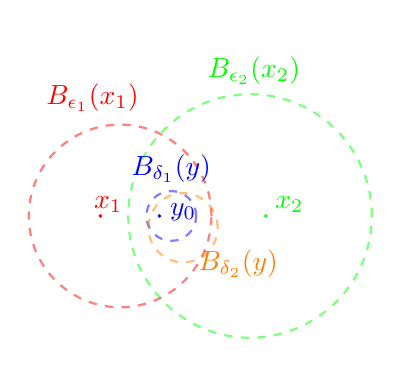
\begin{tikzpicture}[scale = 0.5]
    \draw[red, semitransparent, dashed, thick] (-1,0) circle[radius=66pt];
    \node[label, red] at (-1.7,3) {$B_{\epsilon_1}(x_1)$};
    \node[label, red] at (-1.3, 0.3) {$x_1$};
    \node[circle, fill, red, inner sep=0.5pt] at (-1.5, 0) {};
    \draw[green, semitransparent, dashed, thick] (2.3,0) circle[radius=88pt];
    \node[label, green] at (2.4, 3.7) {$B_{\epsilon_2}(x_2)$};
    \node[label, green] at (3.3, 0.3) {$x_2$};
    \node[circle, fill, green, inner sep=0.5pt] at (2.7, 0) {};
    \draw[blue, semitransparent, dashed, thick] (0.3,0) circle[radius=18pt];
    \node[label, blue] at (0.3, 1.2) {$B_{\delta_1}(y)$};
    \node[label, blue] at (0.6, 0.1) {$y_0$};
    \node[circle, fill, blue, inner sep=0.5pt] at (0, 0) {};
    \draw[orange, semitransparent, dashed, thick] (0.6,-0.3) circle[radius=25pt];
    \node[label, orange] at (2, -1.2) {$B_{\delta_2}(y)$};
    \end{tikzpicture}
    \end{center}
    \end{minipage}
    
    so that $B_{\delta_1}(y) \subset B_{\epsilon_1}(x_1)$. Similarly, setting $\delta_2 = \epsilon_2 - d(x_2, y)$ gives $B_{\delta_2}(y) \subset B_{\epsilon_2}(x_2)$. Let
        $$\delta = \text{min}\left\{\delta_1, \delta_2\right\}$$
    Then
    $$B_{delta}(y) \subset B_{\epsilon_1}(x_1) \cap B_{\epsilon_2}(x_2)$$
\end{proof}

\begin{customdefinition}{4.2}[Metrizable]
A topological space $X$ is called metrizable if there exists a metric $d$ on $X$ whose associated metric topology agrees with that of $X$.\\
Metrizability of a topological space is a subtle problem, but is ultimately known via Urysohn's Metrization Theorem.
\end{customdefinition}

\begin{customdefinition}{4.3}
Let $(X, d)$ be a metric space.
\begin{enumerate}
    \item[1).] A subset $A \subset X$ is called bounded if there exists an $N>0$ such that $d(a_1, a_2) \leqslant N$ for all $a_i \in A$.
    \item[2).] The diameter of a non-empty bounded subset $A\subset X$ is 
                $$\text{diam} A = \text{sup} \left\{d(a_1, a_2) \mid a_i \in A\right\}.$$
\end{enumerate}
\end{customdefinition}

\begin{customthm}{4.2}
Let $(X, d)$ be a metric space. Then define $\overline{d}: X\times X \longrightarrow \R$ by
    $$\overline{d} = \text{min} \left\{d(x,y), 1\right\}$$
in other words
    \begin{align*}
        \overline{d}: X\times X &\longrightarrow \R\\
        (x,y) &\longrightarrow \text{min} \left\{d(x,y), 1\right\}
    \end{align*}
Then $\overline{d}$ is a metric that includes the same topology as $d$.
\end{customthm}

\begin{customthm}{4.3}
The following statements hold.
\begin{enumerate}
    \item[1).] Subspaces of metric space are metrizable.
    \item[2).] Metrizable spaces are Hausdorff.
\end{enumerate}
In particular, Lemma $2.19$ and the $2)$ imply that, if a sequence $x_n$ in a metric space converges, then if has a unique limit.
\end{customthm}

\begin{proof}
\begin{enumerate}
    \item[1).] Let $(X, d)$ be a metric space and $A \subset X$ a subspace. We claim that
                $$d_{\vert A}: A \times A \longrightarrow \R$$
                is a metric on $A$ and that the metric topology on $A$ agrees with the subspace topology. That $d_{\vert A}$ is a metric follows immediately from the metric axioms hold. For the second, we wish to apply Lemma $2.3$. Let
                $$\mathcal{A} =\left\{\underbrace{B_{\epsilon}(y)}_{\text{ with respect to $d_{\vert A}$}} \subset Y \mid y \in Y,\, \epsilon > 0\right\}$$
                (This is the set $\mathcal{C}$ in Lemma $2.3$). Note that 
                $$B_{\epsilon}(y) = \underbrace{B_{\epsilon}}_{\text{open in $X$}}\left(y;d\right) \cap Y$$
                So that $B_{\epsilon}(y) \subset Y$ is open. Let $U \subset Y$ be open and $u \in U$. Then
                $$U = \underaccent{i}{\bigcup}\left(B_{\epsilon_i}(x_i, d) \cap Y\right)$$
                for some $i$. Then 
                $$u \in B = B_{\epsilon_i - d(x_i, u)}(u) \subset U.$$
                Lemma $2.3$ therefore applies, proving the second statement.
    \item[2).] Let $(X, d)$ be a metric space and $x, y \in X$ distinct points. Let $\epsilon = d(x,y) >0$(by the non-negativity axiom). Then $x \in B_{\epsilon/2}(x)$ and $y \in B_{\epsilon/2}(y)$ and 
                $$B_{\epsilon/2}(x) \cap B_{\epsilon/2}(y) = \varnothing$$
                (by the Triangle Inequality). So, $(X,d)$ is Hausdorff.
\end{enumerate}
\end{proof}

\begin{customthm}{4.4}
Finite products of metrizable topological spaces are metrizable.
\end{customthm}

\begin{customthm}{4.5}
Let $(X, d)$ and $(Y, e)$ be metric spaces. A function $f: X \longrightarrow Y$ is continuous if and only if for each $x \in X$ and $\epsilon >0$, there exists a $\delta >0$ such that 
        $$e\left(f(x), f(y)\right) < \epsilon$$
    whenever $d(x,y) < \delta$.\\
    In other words,
        $$d_{X}(x,y) < \delta \implies d_{Y} \left(f(x), f(y)\right) < \epsilon$$
Continuous functions between metric spaces admit an $\epsilon - \delta$ characterization, just like in analysis.
\end{customthm}

\begin{customlemma}{4.6}
Let $A \subset X$ be a subset of a topological space.
\begin{enumerate}
    \item[1).] If $\left\{x_n\right\}_{n \geqslant 0}$ is a sequence in $A$ converging to a point $x$, then $x \in \overline{A}$.
    \item[2).] If $X$ is metrizable and $x \in \overline{A}$, then there exists a sequence $\left\{x_n\right\}_{n \geqslant 0}$ in $A$ converging to $x$.
\end{enumerate}
\end{customlemma}

\begin{customthm}{4.7}
Let $f: X \longrightarrow Y$ be a function between topological spaces.
\begin{enumerate}
    \item[1).] If $f$ is continuous and $\left\{x_n\right\}_{n \geqslant 1}$ converges to $x$, then $\left\{f(x_n)\right\}_{n \geqslant 1}$ converges to $f(x)$.
    \item[2).] If $X$ is metrizable $\left\{f(x_n)\right\}_{n \geqslant 1}$ converges to $f(x)$ for all sequences ${x_n}_n$ converging to $x$, then $f$ is continuous.
\end{enumerate}
\end{customthm}

\newpage

\begin{proof}
\begin{enumerate}
    \item[1).] Let $\left\{x_n\right\}_{n \geqslant 1}$ converges to $x \in X$ and $U \subset Y$ be an open set containing $f(x)$. Since $f$ is continuous, $f^{-1}(U) \subset X$ is open and, by construction, contains $x$. Hence, there exists an $N>0$ such that $x_n \in f^{-1} (U)$ whenever $n >N$. But then $f(x_n) \in U$ whenever $n>N$. So, $\left\{f(x_n)\right\}_{n \geqslant 1}$ converges to $f(x)$.
    \item[2).] Let $(X, d)$ be a metric space and $\left\{x_n\right\}_{n \geqslant 1}$ a convergent sequence, say $x = \displaystyle\lim_{n \to \infty} x_n$. (Note: Since $X$ is metrizable, $\left\{x_n\right\}_{n \geqslant 1}$ converges to a unique point, so that we can safely write $\displaystyle\lim_{n \to \infty} x_n$).\\
    Recall that $f$ is continuous if and only if 
    $$f\left(\overline{A}\right) \subset \overline{f(A)}$$
    for all $A\subset X$; see Theorem $3.2$. Let $x\in \overline{A}$. By Lemma $4.6$, there exists $\left\{x_n\right\}_{n \geqslant 1}$ with $x = \displaystyle\lim_{n \to \infty} x_n$. By hypothesis, $\left\{f(x_n)\right\}_{n \geqslant 1}$ converges to $f(x)$, that is, $f(x) \in \overline{f(A)}$, again by Lemma $4.6$.
\end{enumerate}
\end{proof}

\begin{customdefinition}{4.4}
Let $(X, d)$ be a metric space.
\begin{enumerate}
    \item[1).] A sequence $\left\{x_n\right\}_{n \geqslant 1}$ is called Cauchy if for all $\epsilon > 0$ there exists an $N > 0$ such that 
                $$d(d_n, d_{n+1}) < \epsilon$$
                whenever $m, n > N$
    \item[2).] $(X, d)$ is called complete if every Cauchy sequence converges.
\end{enumerate}
\end{customdefinition}

\begin{customexa}{4.1}The following are examples about complete metric space.
\begin{enumerate}
    \item[1).]$\left(\R, d_E\right)$ is complete;
    \item[2).]$(0,1)$ is not complete, for example
    $$\left\{\dfrac{1}{n}\right\}_{n \geqslant 1}\text{ is Cauchy but does not converge in }(0,1).$$
\end{enumerate}
\end{customexa}

\phantomsection
\subsection*{2. The Quotient Topology}
\addcontentsline{toc}{subsection}{2. The Quotient Topology}

\begin{customdefinition}{4.5}[Equivalence Relationship]
Let $X$ be a set. An equivalence relation on $X$ is $x \sim y$, such that
\begin{enumerate}
    \item[1).] (Reflexivity) $x \sim x$, 
    \item[2).] (Symmetry) $x \sim y$ if and only if $y \sim x$,
    \item[3).] (Transitivity) If $x \sim y$ and $y \sim z$, then $x \sim z$.
\end{enumerate}
The equivalence class of $x$ is 
$$[x] = \left\{y \in X \mid x \sim y\right\} \subset X$$
So 
$$X = \underaccent{x \in X/\sim}{\bigsqcup}[x]$$ 
where $X/\sim = \left\{\text{set of all equivalence classes}\right\}$.
\end{customdefinition}

\begin{customdefinition}{4.6}[Quotient Topology]
Let $X$ be a topological space, $Y$ a set and 
$$q: X\longrightarrow Y$$
a surjective function. The quotient topology on $Y$ (induced by the function $q$) is 
$$\tau_q = \left\{U \subset Y \mid q^{-1}(U) \subset X \text{ is open }\right\}$$
We call $(Y, \tau_q)$ the quotient topological space.\\
\end{customdefinition}

\begin{proof}
We should check this is indeed a topology:
\begin{enumerate}
    \item[1.)] $\varnothing \in \tau_q$ because $q^{-1}(\varnothing) = \varnothing \in \tau$ (topology on $X$). And $Y \in \tau_q$ because $q^{-1}(Y) = X \in \tau$ ($q$ is surjective.)
    \item[2.)] Let $\{U_i\}_{i\in I}$ be an arbitrary collection in $\tau_q$. Then 
    $$q^{-1}\left(\underaccent{i \in I}{\bigcup}U_i\right) = \underbrace{\underaccent{i \in I}{\bigcup} \underbrace{q^{-1}\left(U_i\right)}_{\text{ open in }X}}_{\text{ open in} X} \in \tau_q$$
    \item[2.)] Let $\{U_i\}_{i\in I}$ be a finite collection in $\tau_q$. Then 
    $$q^{-1}\left(\underaccent{i \in I}{\bigcap}U_i\right) = \underbrace{\underaccent{i \in I}{\bigcap} \underbrace{q^{-1}\left(U_i\right)}_{\text{ open in }X}}_{\text{ open in} X} \in \tau_q$$
\end{enumerate}
\end{proof}

\begin{customexa}{4.2}Let $X = \R$. Define an equivalence relation on $X$ by
    $$x \sim y \iff x - y \in \mathbb{Q}$$
    Consider the quotient $X/\sim$. The points $[0], [\pi] \in X/\sim$ are distinct. Let
    $$[0] \in U, \,\, [\pi] \in V$$
    be open sets in (in $X/\sim$). Then $q^{-1}(U) \subset \R$ is an open set which contains $\mathbb{Q}$ and $q^{-1}(V) \subset \R$ is an open set which contains 
    $$\pi + \mathbb{Q} = \left\{\pi + r \mid r \in \mathbb{Q}\right\}$$
    But then $q^{-1}(U) \cap q^{-1}(V) \neq \varnothing$. So, $U \cap V \neq \varnothing$, and $X/\sim$ is not Hausdorff. This example shows that quotient spaces do not, in general inherit the Hausdorff property.
\end{customexa}

\begin{customdefinition}{4.7}[Quotient Map]
Let $X$ and $Y$ be topological spaces; let $f: X\longrightarrow Y$ be a surjective map. The map $f$ is said to be a quotient map provided a subset $U$ of $Y$ is open in $Y$ if and only if $p^{-1}(U)$ is open in $X$.
\end{customdefinition}

\begin{customdefinition}{4.8}[Saturated]
Let $f: X \longrightarrow Y$ be a surjective map of topological spaces. A subset $S \subset X$ is called saturated (with respect to $f$) is any $y \in Y$ which satisfies 
$$S \cap f^{-1}\left(\{y\}\right) \neq \varnothing$$
also satisfies 
$$f^{-1}\left(\{y\}\right) \subset S$$
\emph{Book:} We say that a subset $C$ of $X$ is saturated (with respect to the surjective map $p: X\longrightarrow Y$) if $C$ contains every set $p^{-1} \left(\{y\}\right)$ that it intersects. Thus $C$ is saturated if it equals the complete inverse image of a subset of $Y$. To say that $p$ is a quotient map is equivalent to saying that $p$ is continuous and $p$ maps \emph{saturated} open sets of $X$ to open sets of $Y$ (or saturated closed sets of $X$ to closed sets of $Y$).\\
\emph{More:} A set $X$ is saturated if
    $$S = \underaccent{y\in q(S)}{\bigcup}f^{-1}\left(\{y\}\right)$$
\end{customdefinition}

\begin{customlemma}{4.8}
Let $q: X \longrightarrow Y$ be a continuous surjection. Then $q$ is a quotient map if and only if whenever $V \subset X$ is open and saturated, $q(V) \subset Y$ is open.
\end{customlemma}

\begin{proof}It's another if-and-only-if, you know the drill...
\begin{enumerate}
    \item[$\Longrightarrow$: ] Assume that $q$ is a quotient map. Then $q$ is continuous. Let $V \subset X$ be open and saturated. We claim that
    $$V = q^{-1}\left(q(v)\right)$$
    Clearly, $V \subset q^{-1}\left(q(v)\right)$. Let $x \in q^{-1}\left(q(v)\right)$, that is, $q(x) \in q(v)$. Then $q^{-1}\left(q(x)\right) \cap V \neq \varnothing$. Since $V$ is saturated, $q^{-1}\left(q(v)\right) \subset V$. Or
    $$V = \underaccent{y\in q(V)}{\bigcup}q^{-1}\left(\{y\}\right)$$
    So that 
    $$V = q^{-1}\left(q(v)\right)$$
    Since $q$ is a quotient map and $q^{-1}\left(q(v)\right)$ is open, we know $q\left(V\right) \subset Y$ is open.
    
    \item[$\Longleftarrow$: ]Assume that $q$ is continuous and, if $V \subset X$ is open and saturated, then $q(V)$ is open . Let $U \subset Y$ be a subset such that $q^{-1}(U)$ is open; we need to show that $U \subset Y$ is open. Since $q\left(q^{-1}(U)\right) = U$, it suffices to show that $q^{-1}(U)$ is saturated. Say $y \in Y$ satisfies $q^{-1}\left(\{y\}\right) \cap q^{-1}(U) \neq \varnothing$. Then $y \in U$ and $q^{-1}\left(\{y\}\right) \subset q^{-1}(U)$
\end{enumerate}
\end{proof}

\begin{customthm}{4.9}
Let $g: X \longrightarrow Y$ be a quotient map and $Z$ a topological space. If $f: X \longrightarrow Z$ is continuous and takes a single value in each $g^{-1}\left(\{y\}\right)$, $y \in Y$, then $f$ determines a (unique) continuous function
$$\widetilde{f}: Y \longrightarrow Z$$
such that 
$$f: \widetilde{f} \circ g$$
In pictures:
    \begin{center}
    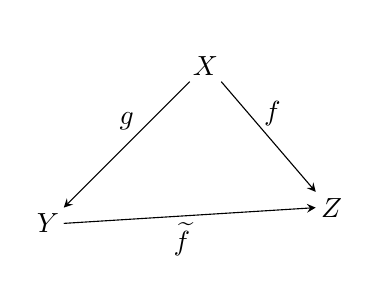
\begin{tikzpicture}
    \node[label] at (0,1) {$X$};
    \node[label] at (1.6,-0.8) {$Z$};
    \node[label] at (-2,-1) {$Y$};
    \draw[-stealth](0.2,0.8) -- (1.4,-0.6);
    \draw[-stealth](-0.2,0.8) -- (-1.8,-0.8);
    \draw[-stealth](-1.8,-1) -- (1.4,-0.8);
    \node[label] at (0.85,0.4) {$f$};
    \node[label] at (-1,0.3) {$g$};
    \node[label] at (-0.3,-1.2) {$\widetilde{f}$};
    \end{tikzpicture}
    \end{center}
\end{customthm}

\begin{proof}(Tells you the quotient definition is the right one.)\\
Let $f: X \longrightarrow Z$ be continuous and constant in each $q^{-1}\left(\{y\}\right)$. So, $f$ takes a single value, $z_y \in Z$, in $q^{-1}\left(\{y\}\right)$. Define
\begin{align*}
    \widetilde{f}: &Y \longrightarrow Z\\
    & y \longmapsto z_y
\end{align*}
Then $f = \widetilde{f} \circ g$. Let $U \subset Z$ be open; want $\widetilde{f}^{-1}(U) \subset Y$ is open. Because $U \subset Z$ open, and $f$ is continuous
$$f^{-1}(U) \subset X$$
is open. Then
$$f^{-1}(U) = q^{-1} \left(\widetilde{f}^{-1}(U)\right)$$
Because $q$ is a quotient map and $f^{-1}(U)$ is open, $\widetilde{f}^{-1}(U)$ is open.
\end{proof}

\begin{customthm}{4.10}
Let $p: X \longrightarrow Y$ be a quotient map; let $A$ be a subspace of $X$ that is saturated with respect to $p$; let $q : A \longrightarrow p(A)$ be the map obtained by restricting $p$.
\begin{enumerate}
    \item[1).] If $A$ is either open or closed in $X$, then $q$ is a quotient map.
    \item[2).] If $p$ is either an open map or a closed map, then $q$ is a quotient map.
\end{enumerate}
\end{customthm}

\newpage
\phantomsection
\section*{5. Connectedness and Compactness}
\addcontentsline{toc}{section}{5. Connectedness and Compactness}

\phantomsection
\subsection*{1. Connectedness}
\addcontentsline{toc}{subsection}{1. Connectedness}

\begin{customdefinition}{5.1}[Connected]
A topological space $X$ is called connected if it {\bf cannot} be written as a union of disjoint non-empty open sets, $U_1, U_2 \subset X$.\\
\emph{Book:} Let $X$ be a topological space. A {\bf separation} of $X$ is a pair $U, V$ of disjoint nonempty open subsets of $X$ whose union is $X$. The space $X$ is said to be {\bf connected} if there does not exist a separation of $X$.\\
\emph{Another Way:} A space $X$ is connected if and only if the only subsets of $X$ that are both open and closed in $X$ are the empty set and $X$ itself.\\
\emph{Extra Comment:} So, to prove that $X$ is connected, assume that 
$$X = U_1 \cup U_2$$
with $U_1, U_2 \subset X$ disjoint and open, and then prove that $U_1 = \varnothing$ or $U_2 = \varnothing$.
\end{customdefinition}

\begin{customthm}{5.1}
The closed interval $[0, 1]$ is connected (in Euclidean topology). More generally, the intervals $(a, b),\,[a, b],\,(a, b],\,[a, b)$, with $-\infty \leqslant a < b \leqslant \infty$, are connected. In fact, those are the only connected subsets of $\R$. 
\end{customthm}

\begin{customthm}{5.2}
Let $U \subset \R$ (with its subspace topology) be connected. Then $U$ is one of the intervals from theorem $5.1$. 
\end{customthm}

\begin{proof}
It suffices to prove that if $a, b \in U$, then $[a, b] \subset U$. Suppose that $c \in [a, b]$ is not in $U$. The sets
$$V_1 = (-\infty, c) \cap U, \,\,\,\, V_2 = (c, \infty) \cap U$$
are then open, disjoint and satisfy $V_1 \cup V_2 = U$. Since $U$ is connected, $V_1 = \varnothing$ or $V_2 = \varnothing$, a contradiction, as $a \in V_1$ and $b \in V_2$.
\end{proof}

\begin{customthm}{5.3}
A topological space $X$ is connected if and only if the only subsets of $X$ which are open and closed are $\varnothing, X$.
\end{customthm}

\begin{proof}
Assume that $X$ is connected and $U \subset X$ is open and closed. Then $X = U \cup (X \setminus U).$ Note that $U\cap (X \setminus U) = \varnothing$ and $X \setminus U$ is open. Since $X$ is connected, $U = \varnothing$ or $U = X$.\\
Conversely, assume that $X$ is such that the only open sets are $\varnothing$ or $X$. Say $X = U_1 \cup U_2$ for disjoint open sets $U_i \subset X$. Then $X \setminus U_1 = U_2$ is closed. Hence, $U_2 = \varnothing$ or $U_2 = X$; in the latter case $U_1 = \varnothing$.
\end{proof}

\begin{customthm}{5.4}
Let $f: X \longrightarrow Y$ be continuous function. If $X$ is connected, the image of $f$, $\left\{f(x) \mid x \in X\right\} \subset Y$, is connected.
\end{customthm}

\begin{customcoro}{5.5}[Intermediate Value Theorem]
Let $f: X \longrightarrow \R$ be a continuous function. Assume that $X$ is connected. If $a, b \in f(x)$, then 
$$[a, b] \subset f(x).$$
\emph{Book:} Let $f: X \longrightarrow Y$ be a continuous map, where $X$ is a connected space and $Y$ is an ordered set in the order topology. If $a$ and $b$ are two points of $X$ and if $r$ is a point of $Y$ lying between $f(a)$ and $f(b)$, then there exists a point $c$ of $X$ such that $f(c) = r$. \\
The intermediate value theorem of calculus is the special case of this theorem that occurs when we take $X$ to be a closed interval in $\R$ and $Y$ to be $\R$.
\hypertarget{Corollary_5.5}{\hyperlink{ex.c.5.5}{Click here for examples.}}
\end{customcoro}

\begin{customcoro}{5.6}The quotient of connected topological space is connected. \hypertarget{Corollary_5.6}{\hyperlink{ex.c.5.6}{Click here for examples.}}
\end{customcoro}

\begin{customdefinition}{5.2}[Connected Components]Let $X$ be a topological space. Define an equivalence relation $\sim$ on $X$ by 
\begin{center}
    $x \sim y$ if there exists $A \subset X$ connected such that $x,y \in A$
\end{center}
The equivalence class of $\sim$ are called connected components of $X$.\\
\emph{Book:} Given $X$, define an equivalence relation on $X$ by setting $x \sim y$ if there is a connected subspace of $X$ containing both $x$ and $y$. The equivalence classes are called the {\bf components} (or the ``connected components") of $X$.\\
\emph{Comment:} Note that a space $X$ is connected is and only if it has a single connected component. So, $[0, 1]$ has one connected component, while $[0, 1] \cup [2,3]$ has two.
\end{customdefinition}

\begin{proof}
Symmetry and reflexivity of the relation are obvious. Transitivity follows by noting that if $A$ is a connected subspace containing $x$ and $y$, and if $B$ is a connected subspace containing $y$ and $z$, then $A \cup B$ is a subspace containing $x$ and $z$ that is connected because $A$ and $B$ have the point $y$ in common. \\
Or to be cooler: Let $U, V \subset A \cup B$ be open and disjoint such that 
$$U \cup V = A \cup B.$$
Assume without loss of generality that $y \in U$. Then 
$$U \cap A \neq \varnothing, \,\,\, U \cap B \neq \varnothing$$
Then 
$$A = \left(U \cap A\right) \cup \left(V \cap A\right), \,\,\, B = \left(U \cap B\right) \cup \left(V \cap B\right)$$
Since $A$ is connected, $V \cap A = \varnothing$, that is, $V \subset B$. But then $U \cap B = \varnothing$, as $B$ is connected. This is a contradiction.
\end{proof}

\begin{customthm}{5.7}
Let $X,\, Y$ be connected topological spaces. Then $X \times Y$ is connected.
\hypertarget{Theorem_5.7}{\hyperlink{ex.t.5.7}{Click here for examples.}}
\end{customthm}

\begin{customthm}{5.8}
The connected components of a topological space $X$ are connected disjoint subspaces of $X$ whose union is $X$, such that each nonempty connected subspace of $X$ intersects only one of them.\\
\emph{Comment:} A {\bf stronger version} is the connected components of a topological space $X$ are connected disjoint subspaces of $X$ whose union is $X$, such that each nonempty connected subspace of $X$ {\bf lies} in exactly one connected component.
\end{customthm}

\begin{proof}
The construction of connected components as equivalence classes implies that they are pairwise disjoint and cover $X$.\\
Let $U \subset X$ be connected. Say $U$ intersects two connected components $C_1$ and $C_2$. Then $C_1 \cap C_2 \neq \varnothing$ so that $C_1 = C_2$.\\
We need to check that each connected component $C$ is connected. Fix $x \in C$. if $y \in C$, then there exists a connected subset $A_y \subset X$, such that 
$$x, y \in A_u\,\,\, (\implies x \sim y)$$
Then 
$$C \subset \underaccent{y\in C}{\bigcup} \underbrace{A_y}_{\text{connected}}$$
And by the result just proved, $A_y \subset C$. Therefore,
$$C = \underaccent{y\in C}{\bigcup} A_y$$
\end{proof}

\begin{customdefinition}{5.3}[Path Connectedness]Let $X$ be a topological space. \hypertarget{Definition_5.3}{\hyperlink{ex.d.5.3}{Click here for examples.}}
\begin{enumerate}
    \item[1).] A {\bf path} in $X$ is a continuous function $f: [a,b] \longrightarrow X$ for some $-\infty < a < b < \infty$.
    \item[2).] Call $X$ {\bf path connected} if, for each $x, y \in X$, there exists a path from $x$ to $y$, that is, a path $f: [a,b] \longrightarrow X$ such that $f(a) = x$, $f(b) = y$.
    \item[3).] The {\bf path components} of $X$ are the equivalence classes of $X$ under the equivalence relation
    \begin{center}
        $x \sim y$ if there exists a path from $x$ to $y$.
    \end{center}
\end{enumerate}
\end{customdefinition}

\phantomsection
\subsection*{2. Compactness}
\addcontentsline{toc}{subsection}{2. Compactness}

\begin{customdefinition}{5.4}[Open Cover]Let $X$ be a topological space. 
\begin{enumerate}
    \item[1).] An {\bf open cover} of $X$ is an arbitrary collection $\left\{U_i\right\}_{i \in I}$ of open subsets of $X$ such that
    $$\underaccent{i \in I}{\bigcup} U_i = X.$$
    \item[2).] A {\bf subcover} of an open cover $\left\{U_i\right\}_{i \in I}$ is a subset $J \subset I$ such that $\left\{U_j\right\}_{j \in J}$ is an open cover of $X$.
    \item[3).] A {\bf finite subcover} of an open cover is a subcover as in $2)$ with $J$ a finite set. (A {\bf finite subcover} subcover is a subcover with $|J| < \infty$.)
\end{enumerate}
\end{customdefinition}

\begin{customdefinition}{5.5}[Compactness] \hypertarget{Definition_5.5}{\hyperlink{ex.d.5.5}{Click here for examples.}}\\
A topological space $X$ is called {\bf compact} if every open cover of $X$ has a finite subcover.\\
\emph{Book:} A space $X$ is said to be {\bf compact} if every open covering $\mathcal{A}$ of $X$ contains a finite subcollection that also covers $X$.\\
\emph{Comment:} Really difficult to construct examples using this definition. Since it may be easy to show a space is non-compact using it.
\end{customdefinition}

\begin{customthm}{5.9}
If $X$ is compact and $C \subset X$ is a closed subset, then $C$ is compact.\\
\emph{Recall:} If $Y$ is a subspace of $X$, a collection $\mathcal{A}$ of subsets of $X$ is said to {\bf cover} $Y$ if the union of its elements contains $Y$.
\end{customthm}

\begin{proof}
Let $\left\{U_i\right\}_{i \in I}$ be an open cover of $C$. Then $U_i = \widetilde{U}_i \cap C$ for some open subset $\widetilde{U}_i \subset X$. Then 
$$\left\{X \setminus C\right\} \cup \left\{\widetilde{U}_i\right\}_{i \in I}$$
is an open cover of $X$. (Since $C$ is closed, $X \setminus C$ is open.) \\
Since $X$ is compact, there is a finite subcover, say 
$$\left\{X \setminus C\right\} \cup \left\{\widetilde{U}_j\right\}_{j \in J},$$
with $J\subset I$ finite. Then $\left\{U_j\right\}_{j \in J}$ is a finite subcover of $\left\{U_i\right\}_{i \in I}$, and $C$ is compact.
\end{proof}

\begin{customthm}{5.10}
Let $X$ be Hausdorff. If $C \subset X$ is a compact subspace, then $C$ is closed.\\
\emph{Comment:} This the converse of the previous theorem is true only if we made $X$ Hausdorff.
\end{customthm}

\begin{proof}
We prove that $X \setminus C \subset X$ is open. Let $x \in X \setminus C$, want an open set $W \subset X$ such that $x \in W \subset X \setminus C$. For each $c \in C$, there exists open sets 
$$c \in U_c, \,\,\, x \in V_c$$
and 
$$U_c \cap V_c = \varnothing$$
Then $\left\{U_c \cap C\right\}_{c \in C}$ is an open cover of $C$. By compactness, there exists $C_1, \dots, C_n \in C$ such that 
$$\left\{U_{C_i} \cap C\right\}_{i = 1, \dots, n}$$
covers $C$ (finite subcover). Then 
$$W = V_{C_1} \cap \dots \cap V_{C_n}$$
is an open subset of $X$ which contains $x$ and is disjoint from $C$. Note that $x \in V$ and $W$ is open. So, $x \in W \subset X \setminus C$, proving that $X \setminus C$ is open.
\end{proof}

\begin{customthm}{5.11}
Let $f: X \longrightarrow Y$ be continuous function with $X$ is compact. Then $f(X) \subset Y$ is compact. 
\end{customthm}

\begin{proof}
Let $\left\{U_i\right\}_{i \in I}$ and open cover of $f(X)$. Write 
$$U_i = \widetilde{U}_i \cap f(X)$$
for some $\widetilde{U}_i \subset Y$ is open. Then 
$$\left\{f^{-1}\left(\widetilde{U}_i\right)\right\}_{i \in I}$$
is an open cover of $X$. By compactness of $X$, there is a finite subcover 
$$\left\{f^{-1}\left(\widetilde{U}_j\right)\right\}_{j \in J}$$
Then 
$$\left\{U_j\right\}_{j \in J}$$
is a finite subcover of $f(X)$.
\end{proof}

\begin{customthm}{5.12}
For any $a < b$, the closed interval $[a, b] \subset \R$ is compact. (Proof is pretty insane, will come back when having more time.)
\end{customthm}

\begin{customthm}{5.13}[Heine-Borel]
A subset of $\R$ is compact if and only if it is closed and bounded.
\end{customthm}

\begin{customthm}{5.14}[The Theorem of Life Appreciation]
\addcontentsline{toc}{subsection}{(The Theorem of Life Appreciation)}
\hypertarget{Theorem_5.14}{\hyperlink{ex.t.5.14}{Click here for examples.}}\\
Let $f : X \longrightarrow Y$ be a continuous function which is bijective. If $X$ is compact and $Y$ is Hausdorff, than $f^{-1}$ is continuous. So $f$ is a homeomorphism.
\end{customthm}

\begin{proof}(Would be a shame to not give it a proof)\\
We need to show that the images of closed sets of $X$ under $f$ are closed in $Y$, this will prove the continuity of the map $f^{-1}$. Let $C \subset X$ be closed. Since $X$ is compact, so is $C$ (Theorem, $5.9$). Then $f(C) \subset Y$ is compact (Theorem $5.11$). Since $Y$ is Hausdorff, $f(C)$ is closed (Theorem $5.10$).
\end{proof}

\begin{customthm}{5.15} Let $X, Y$ be compact topological spaces. Then $X \times Y$ is compact. (Proof is again pretty insane, will come back when having more time.)
\end{customthm}

\begin{customcoro}{5.16}The following topological spaces are compact:
\begin{enumerate}
    \item[1).] $[0,1]^n$ for each $n \geqslant 1$.
    \item[2).] The $n$-sphere $S^n = [0,1]^n / _{\partial [0, 1]^n}$ for each $n \geqslant 1$.
    \item[3).] The $n$-torus $\Pi^n = \left(S^1\right)^n$ for each $n \geqslant 2$.
    \item[4).] The real projective spaces $\mathbb{RP}^n$ for each $n \geqslant 1$.
\end{enumerate}
\end{customcoro}

\begin{proof} The proofs for the previous corollary:
\begin{description}
    \item[1).] This follows from Theorem $5.12$ and $5.15$
    \item[2) $\sim$ 3).] These follow from $1)$ and the fact that the quotient of a compact space is compact (by Theorem $5.11$).
    \item[4).] Consider the $n$-sphere
    $$S^n = \left\{\left(x_1, \dots, x_{n+1} \right) \in \R^{n+1} \Big| \ds\sum_{i = 1}^{n +1} \left(x_i\right)^2 = 1 \right\}$$
    Define an equivalence relation on $S^n$ by 
    $$p \sim -p, \,\,\, p \in S^n$$
    (Note: Equivalence classes in $S^n$ are the antipodal points.) The quotient space $S^n /_{\sim}$ is $\mathbb{RP}^n$. It is compact since $S^n$ is. (To use that $S^n$ is compact, one can prove that $[0,1]^n / _{\partial [0, 1]^n} \simeq S^n$) using Theorem $5.14$ or use that $S^n \subset \R^{n+1}$ is closed and bounded and apply Heine-Borel.)
\end{description}
\end{proof}

\begin{customthm}{5.17}[Extreme Value Theorem] Let $f: X \longrightarrow \R$ be a continuous function. If $X$ is compact, then there exist points $x_m, x_M \in X$ such that 
$$f\left(x_m\right) \leqslant f(x) \leqslant f\left(x_M\right) , \,\,\,\,\, x \in X.$$
\end{customthm}

\begin{proof}
The image $f(X) \subset \R$ is compact, by Theorem $5.11$. We show that $f(X)$ has a maximal element $M$ and then choose $x_M \in X$ such that $f\left(x_M\right) = M$. Let's proceed by contradiction. In this case, if $f(X)$ has no largest element, the collection 
    $$\left\{(-\infty, y) \cap f(X) \mid y \in f(X)\right\}$$
is an open cover of $f(X)$. By compactness, there exists $y_1 < \dots < y_n$ in $f(X)$ such that 
    $$\left\{(-\infty, y_i) \cap f(X) \mid i = 1, \dots, n\right\}$$
covers $f(X)$. But then $y_{n} \notin f(X)$, a contradiction.
\end{proof}

\begin{customdefinition}{5.6}[Distance]
Let $(X, d)$ be a metric space and $A \subset X$ a non-empty subset. The {\bf distance} from $x \in X$ to $A$ is 
$$d(x, A) = \text{inf}\left\{d(x, a) \mid a \in A\right\}$$
\emph{Comment:} To show that for fixed $A$, the function $d(x, A)$ is a continuous function of $x$: Given $x, y \in X$, one has the inequalities 
$$d(x, A) \leqslant d(x, a) \leqslant d(x, y) + d(y, a),$$
for each $a \in A$. It follows that 
$$d(x, A) - d(x,y) \leqslant \text{inf} d(y, a) = d(y, A),$$
so that 
$$d(x, A) - d(y, A) \leqslant d(x, y).$$
The same inequality holds with $x$ and $y$ interchanged; continuity of the function $d(x,A)$ follows. Recall the {\bf diameter} of a bounded subset $A$ of a metric space $(X, d)$ is the number 
$$\text{sup}\left\{d(a_1, a_2) \mid a_1, a_2 \in A\right\}.$$
\end{customdefinition}

\begin{customthm}{5.18}[The Lebesgue Number Lemma] Let $\left\{U_i\right\}_{i \in I}$ be an open cover of a compact metric space $(X, d)$. Then there exists a $\delta > 0$ (called a {\bf Lebesgue Number}) such that each (bounded) subset of $X$ of diameter less than $\delta$ is contained in some $U_i$. (Can't even understand the theorem yet, leave the proof for later)
\end{customthm}

\begin{customdefinition}{5.7}[Uniform Continuity]
A function $f$ from the metric space $(X, d_X)$ to the metric space $(Y, d_Y)$ is said to be {\bf uniformly continuous} if given $\epsilon > 0$, there is a $\delta > 0$ such that for every pair of points $x_0, x_1$ of $X$.
$$d_X\left(x_0, x_1\right) < \delta \implies d_Y\left(f(x_0), f(x_1)\right) < \epsilon.$$
\end{customdefinition}

\begin{customdefinition}{5.8}[Limit Point Compact]
A space $X$ is said to be {\bf limit point compact} if every infinite subset of $X$ has a limit point.
\end{customdefinition}

\begin{customthm}{5.19}Compactness implies limit point compactness, but not conversely.
\end{customthm}

\begin{customdefinition}{5.9}[Sequentially Compact]
Let $X$ be a topological space. If $(x_n)$ is a sequence of points of $X$, and if 
$$n_1 < n_2 < \dots < n_i < \dots $$
is an increasing sequence of positive integers, then the sequence $(y_i)$ defined by setting $y_i = x_{n_i}$ is called a {\bf subsequence} of the sequence $(x_n)$. The space $X$ is said to be {\bf sequentially compact} if every sequence of points of $X$ has a convergent subsequence.
\end{customdefinition}

\begin{customthm}{5.20}Let $X$ be a metrizable space. Then the following are equivalent:
\begin{enumerate}
    \item[1).] $X$ is compact.
    \item[2).] $X$ is limit point compact.
    \item[3).] $X$ is sequentially compact.
\end{enumerate}
\end{customthm}

\newpage
\phantomsection
\section*{6. Surfaces}
\addcontentsline{toc}{section}{6. Surfaces}

\phantomsection
\subsection*{1. Manifolds}
\addcontentsline{toc}{subsection}{1. Manifolds and Complexes}

\begin{customdefinition}{6.1}[Second Countable] 
\hypertarget{Definition_6.1}{\hyperlink{ex.d.6.1}{Click here for examples.}}\\
A topological space $X$ is called {\bf second countable} if it has a countable (remember ``countable", huh? Probably the hard way, eh?) basis for its topology.\\
\emph{Comment:} Like compactness, second countability should be seen as a ``smallness" condition on a topological space.
\end{customdefinition}

\begin{customdefinition}{6.2}[$n$-Dimensional Manifold] 
\hypertarget{Definition_6.2}{\hyperlink{ex.d.6.2}{Click here for examples.}}
\begin{enumerate}
    \item[1)] Let $n \geqslant 1$. An $n-$dimensional (topological) manifold is a topological space $M$ such that 
        \begin{enumerate}
            \item[i)] $M$ is Hausdorff
            \item[ii)] $M$ is second countable
            \item[iii)] $M$ is locally Euclidean: for any $m \in M$, there exists an open set $x \in U \subset M$, an open set $\widetilde{U} \subset \R^n$ and a homeomorphism $\varphi: U \longrightarrow \widetilde{U}$.
        \end{enumerate}
    \item[2)] A {\bf surface} is a $2$-manifold.
\end{enumerate}
\end{customdefinition}

\begin{customdefinition}{6.3}Let $X, Y$ be topological spaces. The disjoint union $X \bigsqcup Y$ is the topological space with set $X \bigsqcup Y$ with $U \subset X \bigsqcup Y$ open if 
$$U \cap X \subset X, \text{ and } \,U \cap Y \subset Y$$
are open.
\end{customdefinition}

\begin{customdefinition}{6.4}[Connected Sum] Let $M, N$ be $n$-manifolds, e.g(exempli gratia), surfaces. The {\bf connected sum} $M\#N$ is the $n$-manifold defined as follows:
\begin{enumerate}
    \item[i)] Pick $a \in M$, an open set $a \in U_a \subset M$ and a homeomorphism $\varphi_a : U_a \xrightarrow{\widesim{}} B_1(0) \subset \R^n$, and similarly for $b \in N$, giving $\left(b, U_b, \varphi_b\right)$. (Note: The sets $U_a$ must be sufficiently nice - ``regular Euclidean")
    \item[ii)] Consider $M \setminus U_a$ and $N \setminus U_b$. The composition 
            $$U_a \xrightarrow{\varphi_a} B_1(0) \xrightarrow{\varphi^{-1}_b} U_b$$
            extends to a homeomorphism 
            $$\Phi: \overline{U}_a \longrightarrow \overline{U}_b$$ 
            sending the boundary $S^{n-1}$ to the boundary $S^{n-1}$.
    \item[iii)] Define 
            $$M \# N = \left(M \setminus U_a\right) \bigsqcup \left(N \setminus U_b\right) /_{\sim}$$
            where 
            $$\partial \overline{U}_a \ni x \sim \Phi(x) \in \partial \overline{U}_b.$$
\end{enumerate}
\emph{Remark: }If $M$ and $N$ are connected, then connected sum is connected. That is $M\# N$ is independent of all choices.
\end{customdefinition}

\begin{customthm}{6.1}
Every compact connected surface is homeomorphic to exactly one of $\left\{\Sigma_g\right\}_{g \geqslant 0}$ or $\left\{N_g\right\}_{g \geqslant 0}$.
\begin{enumerate}
    \item[1.] $\Sigma_g = S^2 \# \underbrace{\Pi^2 \# \Pi^2 \# \dots \# \Pi^2}_{g \text{ times}}$ is called closed orientable surface of genus $g$.
    \item[2.] $N_g = \mathbb{RP}^2\# \underbrace{\mathbb{RP}^2 \# \mathbb{RP}^2 \# \dots \# \mathbb{RP}^2}_{g \text{ times}}$ is called closed non-orientable surface of genus $g$.
\end{enumerate}
\end{customthm}

\begin{customdefinition}{6.5}[Simplex] 
Let $k$ be a positive integer. We say that the vectors $v_0, \dots, v_k$ are in general position, i.e. they do not all lie in an affine $(k -1)$-plane in $\R^n$. For low $k = $
    \begin{enumerate}
        \item[$1$:] The vectors are not equal.
        \item[$2$:] The vectors are not colinear.
    \end{enumerate}
Define the $k$-dimensional simplex, or $k$-simplex spanned by them is 
$$\bigtriangleup^n = \left\{a_0v_0 + a_1v_1 + \dots + a_kv_k \mid 0 \leqslant a_i \leqslant 1, \sum_{i = 0}^{k}a_i = 1\right\}$$
In particular, the standard $k$-simplex is
$$\left\{\left(a_0, \dots, a_k\right) \in \R^{k+1} \mid 0 \leqslant a_i \leqslant 1, \sum_{i = 0}^{k}a_i = 1\right\}$$
\emph{Remark:} A $0$-simplex is a point, a $1$-simplex is a line segment, a $2$-simplex is a triangle, a $3$-simplex is a tetrahedron, and so on.
\end{customdefinition}



\newpage 
\addcontentsline{toc}{part}{Part 2. Counterexamples in Topology}
\phantomsection
\addcontentsline{toc}{chapter}{1. Basic Definitions}
\input{Counterexamples_in_Topology/part_1}
\newpage

\phantomsection
\addcontentsline{toc}{chapter}{2. Counterexamples}
\input{Counterexamples_in_Topology/part_2}

\phantomsection
\addcontentsline{toc}{chapter}{3. Metrization Theory}
\input{Counterexamples_in_Topology/part_3}

\newpage
\addcontentsline{toc}{part}{Appendices}
\phantomsection
\addcontentsline{toc}{chapter}{Appendix 1. Set Theory and Sh*ts}

\phantomsection
\section*{1. Fundamental Concepts}
\addcontentsline{toc}{section}{1. Fundamental Concepts}

\phantomsection
\subsection*{1 Sets}
\addcontentsline{toc}{subsection}{1. Sets}

\begin{enumerate}
    \item[1.]\emph{DeMorgan's Laws}
            \begin{align*}
            A - \left(B \cup C\right) &= \left(A - B\right)\cap \left(A - C\right)\\
            A - \left(B \cap C\right) &= \left(A - B\right)\cup \left(A - C\right)
            \end{align*}
    \item[2.]Verbalized version of the \emph{DeMorgan's Laws}
            \begin{center}
                The complement of the union equals the intersection of the complements.\\
                The complement of the intersection equals the union of the complements.
            \end{center}
    \item[3.]\emph{Distributive Law}
            $$A \cup \left(B \cap C\right) = \left(A\cup B\right)\cap \left(A\cup C\right)$$
    \item[4.]\emph{ Arbitrary Unions and Intersections}
            \begin{enumerate}
                \item[i)] Given a collection $\mathcal{A}$ of sets, the union of the elements of $\mathcal{A}$ is defined by the equation
                $$\underset{A \in \mathcal{A}}{\bigcup} A = \left\{x \mid \, x\in A \text{ for at least one } A \in \mathcal{A}\right\}.$$
                \item[ii)] The intersection of the elements of $\mathcal{A}$ is defined by the equation 
                $$\underset{A \in \mathcal{A}}{\bigcap} A = \left\{x \mid \, x\in A \text{ for every } A \in \mathcal{A}\right\}.$$
            \end{enumerate}
    \item[5.] \emph{Cartesian Products}\\
            Given sets $A$ and $B$, we define their cartesian product $A \times B$ to be the set of all ordered pairs $(a, b)$ for which $a$ is an elements of $A$ and $b$ is an element of $B$. Formally,
            $$A \times B = \left\{(a, b) \mid a \in A \text{ and } b \in B\right\}$$
        \item[6.] \emph{This guy}
        $$(a, b) = \bigcup_{i=1}^{\infty} \left[a - \dfrac{b - a}{i}, b\right)$$
\end{enumerate}

\phantomsection
\subsection*{2. Functions}
\addcontentsline{toc}{subsection}{2. Functions}

\begin{enumerate}
    \item[1.] \emph{Rule of Assignment}\\
    A {\bf rule of assignment} is a subset $r$ of the cartesian product $C \times D$ of two sets, having the property that each element of $C$ appears as the first coordinate of \emph{at most one} ordered pair belonging to $r$. Thus, a subset $r$ of $C \times D$ is a rule of assignment if 
    $$\left[(c,d) \in r \text{ and } (c, d') \in r\right] \implies \left[d = d'\right]$$
    \item[2.] \emph{Domain and the Image Set}\\
    Given a rule of assignment $r$, the {\bf domain} of $r$ is defined to be the subset of $C$ consisting of all first coordinates of elements of $r$, and the {\bf image set} of $r$ is defined as the subset of $D$ consisting of all second coordinates of elements of $r$. Formally,
    \begin{align*}
        \text{domain }r &= \left\{c \mid \text{there exists $d \in D$ such that $(c, d) \in r$}\right\}.\\
        \text{image }r & =\left\{d \mid \text{there exits $c \in C$ such that $(c, d) \in r$}\right\}
    \end{align*}
    \item[3.] \emph{Function}\\
    A {\bf function} $f$ is a rule of assignment $r$, together with a set $B$ that contains the image set of $r$, The domain $A$ of the rule $r$ is also called the {\bf domain} of the function $f$; the image set of $r$ is also called the {\bf image set} of $f$; and the set $B$ is called the {\bf range} of $f$.
    $$f: A \longrightarrow B$$
    \item[4.] \emph{Restriction}\\
    If $f: A \longrightarrow B$ and if $A_0$ is a subset of $A$, we define the {\bf restriction} of $f$ to $A_0$ to be the function mapping $A_0$ into $B$ whose rule is 
    $$\left\{\left(a, f(a)\right) \mid a \in A_0\right\}$$
    It is denoted by $f_{\mid A_0}$, which is read ``$f$ restricted to $A_0$."
    \item[5.] \emph{Composite Function}\\
    Given functions $f: A \longrightarrow B$ and $g: B \longrightarrow C$, we define the {\bf composite} $g \circ f$ of $f$ and $g$ as the function $g \circ f: A \longrightarrow C$ defined by the equation $\left(g \circ f\right)(a) = g\left(f(a)\right)$. Formally, $g \circ f : A \longrightarrow C$ is the function whose rule is 
    $$\left\{(a,c) \mid \text{ For some $c \in B, f(a) = b$ and $g(b) =c$}\right\}.$$
    \item[6.] \emph{Injective, Surjective, Bijective, and Inverse}
    \begin{enumerate}
        \item[i)] A function is $f: A \longrightarrow B$ is said to be {\bf injective} (or {\bf one-to-one}) if for each pair of distinct points of $A$, their images under $f$ are distinct. Formally, $f$ is injective if 
        $$\left[f(a) = f(a')\right] \implies \left[a = a'\right]$$
        \item[ii)] A function is $f: A \longrightarrow B$ is said to be {\bf surjective} (or $f$ is said to map $A$ {\bf onto} $B$) if for every element of $B$ is the image of some element of $A$ under the function $f$. Formally, $f$ is injective if 
        $$\left[b \in B\right] \implies \left[b = f(a) \text{ for at least one } a \in A \right]$$
        \item[iii)] If $f: A \longrightarrow B$ is both injective and surjective, it is said to be {\bf bijective} (or is called a {\bf one-to-one correspondence}).
        \item[iv)] If $f$ is bijective, there exists a function from $B$ to $A$ called the {\bf inverse} of $f$. It is denoted by $f^{-1}$ and is defined by letting $f^{-1}(b)$ be that unique element $a$ of $A$ for which $f(a) = b$.
    \end{enumerate}
    \emph{Comment: }This comment is added solely because the importance it plays in the homework and stuff:\begin{enumerate}
        \item[a).] The composite of two injective functions is injective, and the composite of two surjective functions is surjective; it follows that the composite of two bijective functions is bijective.
        \item[b).] Given $b \in B$, the fact that $f$ is surjective implies that there exists such an element $a \in A$; the fact that $f$ is injective implies that there is only one such element $a$. It is easy to see that if $f$ is bijective $f^{-1}$ is also bijective.
        \item[c).] The inverse of a composite function $\left(g \circ f \right)(a)$ is given by $(g \circ f)^{-1}(a) = f^{-1}\left(g^{-1}(r)\right)$.
        \item[d).] Given that $f:A \longrightarrow B$ and $g: B\longrightarrow C$:
            \begin{itemize}
                \item If $g \circ f$ is injective then $f$ is injective.
                \item If $g \circ f$ is surjective then $g$ is surjective.
            \end{itemize}
            so if $g \circ f$ is bijective then $f$ is injective and $g$ is onto, but the converse is not true.
            \begin{proof} The two bullet points and the comment:
                \begin{itemize}
                    \item $f(x) = f(x') \implies g\left(f(x)\right) = g\left(f(x')\right) \implies \left(g \circ f\right)(x) = \left(g \circ f\right)(x') \implies x = x'$
                    \item If $c \in C$ then $\exists\, a$ such that
                    $$\left(a \in A \land \left(g \circ f\right)(a) = c\right) \implies \left(a' \in A \land g \left(f(a')\right) = c\right)$$
                    Consider $b = f(a) \in B$ then $g(b) = c.$
                    \end{itemize}
            Now take $A = \{1, 2\}, \,B = \{3, 4, 5\}\, C = \{6, 7\}$ and 
            $$f(1)= 3, f(2) = 4; g(3) = g(4) = 6, g(5) = 7$$
            $f$ is injective and $g$ is onto but 
            $$\left(g \circ f\right)(1) = \left(g \circ f\right)(2) = 6$$
            which means that $g\circ f$ is not a bijective map.
            \end{proof}
    \end{enumerate}
    \item[7.] \emph{Image and Preimage}\\
        Let $f: A \longrightarrow B$. If $A_0$ is a subset of $A$, we denote $f(A_0)$ the set of all images of points of $A_0$ under the function $f$; this set is called the {\bf image} of $A_0$ under $f$. Formally,
        $$f(A_0) = \left\{b \mid b = f(a) \text{ for at least one $a \in A_0$}\right\}.$$
        On the other hand, if $B_0$ is a subset of $B$, we denote by $f^{-1}(B_0)$ the set of all elements of $A$ whose images under $f$ lie in $B_0$; it is called the {\bf preimage} of $B_0$ under $f$ (or the ``counterimage," or the ``inverse image," of $B_0$). Formally,
        $$f^{-1}\left(B_0\right) = \left\{a \mid f(a) \in B_0\right\}.$$
        \emph{Comment:} Note that if $f: A \longrightarrow B$ is bijective and $B_0 \subset B$, we have two meanings for the notation $f^{-1}\left(B_0\right)$. It can taken to denote the {\bf preimage} of $B_0$ under the function $f$ or to denote the {\bf image} of $B_0$ under the function $f^{-1}: B \longrightarrow A$. These two meanings give precisely the same subset of $A$, however, so there  is, in fact, no ambiguity.
    \item[8.] $f^{-1}\left(f(A_0)\right)\stackrel{?}{=} A_0$ and $f\left(f^{-1}(B_0)\right)\stackrel{?}{=} B_0$\\
        If $f: A \longrightarrow B$ and if $A_0 \subset A$ and $B_0 \subset B$, then
        $$A_0 \subset f^{-1}\left(f(A_0)\right) \,\,\,\,\,\,\text{ and } \,\,\,\,\,\, f\left(f^{-1}(B_0)\right) \subset B_0.$$
        The first inclusion is an equality if $f$ is injective, and the second inclusion is an equality if $f$ is surjective.
\end{enumerate}

\phantomsection
\subsection*{3. Relations}
\addcontentsline{toc}{subsection}{3. Relations}

\begin{enumerate}
    \item[1.] \emph{Relation}\\
    A {\bf relation} on a set $A$ is a subset $C$ of the cartesian product $A \times A$. A relation $R$ can have the following properties:
        \begin{enumerate}
            \item[i)] (Reflexive) $xRx$ for all $x \in A$;
            \item[ii)] (Symmetric) $xRy \implies yRx$ for all $x, y \in A$;
            \item[iii)] (Transitive) $xRy \land yRz \implies xRz$ for all $x, y, z \in A$;
            \item[iv)] (Antisymmetric) $xRy \land yRx \implies x = y$ for all $x, y, z \in A$;
            \item[v)] (Asymmetric) $xRy \implies y\cancel{R}x$ for all $x, y \in A$;
            \item[vi)] (Irreflexive) $x\cancel{R}x$ for all $x \in A$.
        \end{enumerate}
    with $i) \sim iii)$ defines an {\bf equivalence relation} (usually write $R$ as $\sim$) on set $A$.
    \item[2.] \emph{Equivalence Class}\\
    Given an equivalence relation $\sim$ on a set $A$ and an element $x$ of $A$, we define a certain subset $E$ of $A$, called the {\bf equivalence class} determined by $x$, by the equation 
        $$E = \left\{y \mid y \sim x.\right\}$$
        Note that the equivalence class $E$ determined by $x$ contains $x$, since $x \sim x$.
    \item[3.] \emph{Partition}\\
    A {\bf partition} of a set $A$ is a collection of disjoint nonempty subsets of $A$ whose union is all of $A$.
    \item[4.] \emph{Order Relation}\\
    Not mentioned in class and not really needed for the exams and homework, will come back later to add the information.
\end{enumerate}


\newpage


\newpage
\phantomsection
\addcontentsline{toc}{chapter}{Appendix 2. Examples}

\phantomsection
\section*{5. Connectedness and Compactness}
\addcontentsline{toc}{section}{5. Connectedness and Compactness}

\begin{customexa}{c.5.5} Here is some an example for \hypertarget{ex.c.5.5}{\hyperlink{Corollary_5.5}{Corollary $5.5$ (Intermediate Value Theorem)}}.\\
Let $f: S^1 \longrightarrow \R$ be continuous.\\
Claim: such a function can never be injective. (Borsuk–Ulam theorem)\\
Let 
$$g:S^1 \longrightarrow \R, x \mapsto f(x) - f(-x)$$
Note that $g(x) = -g(-x)$. So, $g$ is either the zero function or not.
    \begin{enumerate}
        \item[1)] If $g = 0$, then $f(x) = f(-x)$ for all $x \in S^1$, then $f$ is not injective.
        \item[2)] If $g \neq 0$, then there exists a $x_* \in S^1$ such that 
        \begin{align*}
            g(x_*) > 0 &\text{ or } g(x_*) < 0\\
            \implies g( -x_*) < 0 &\text{ or } g(-x_*) > 0
        \end{align*}
        By the IVT, there exists a $x_0 \in S^1$ such that $g(x_0) = 0$, which means $f(x_0) = f(-x_0)$, that is, $f$ is not injective.
    \end{enumerate}
\end{customexa}

\begin{customexa}{c.5.6} Here are some examples for \hypertarget{ex.c.5.6}{\hyperlink{Corollary_5.6}{Corollary $5.6$}}.
\begin{enumerate}
    \item[1).] $S^1$ is connected: it is the quotient of $[0,1]$ by an equivalence relation $0 \sim 1$.
    \item[2).] The nasty space $\R/\sim$ is connected even not Hausdorff.
\end{enumerate}
\end{customexa}

\begin{customexa}{t.5.7} Here are some examples for \hypertarget{ex.t.5.7}{\hyperlink{Theorem_5.7}{Theorem $5.7$}}.
\begin{enumerate}
    \item[1).] The $2$-sphere $S^2$ is connected:
    $$[0,1] \times [0,1] /_{\partial\left([0,1] \times [0,1]\right)}$$
    \item[2).] The two dimensional torus is connected:
    $$[0,1] \times [0,1] /_{\sim}$$
    \item[3).] The Klein bottle is connected:
    $$[0,1] \times [0,1] /_{\sim}$$
\end{enumerate}
Click here for the amazing drawings of the three (might update later): \href{https://en.wikipedia.org/wiki/Surface_(topology)}{Classification of Surfaces}
\end{customexa}

\begin{customexa}{d.5.3} Here are some examples for \hypertarget{ex.d.5.3}{\hyperlink{Definition_5.3}{Definition $5.3$ (Path Connectedness)}}.
\begin{enumerate}
    \item[1).] $\R^n$ is connected. Let $X = \R^n$, then $X$ is path connected: given $x, y \in R^n$, the function 
    $$f:[0, 1] \longrightarrow \R^n, \,\,\,\, t \mapsto xt + (1-t)y$$
    is a path from $y$ to $x$.
    \item[2).] Let $X = \R^n \setminus \{0\}$. If $n \geqslant 2$, then $X$ is path connected. In pictures:\\
    \begin{minipage}{0.5\textwidth}
        \begin{center}
        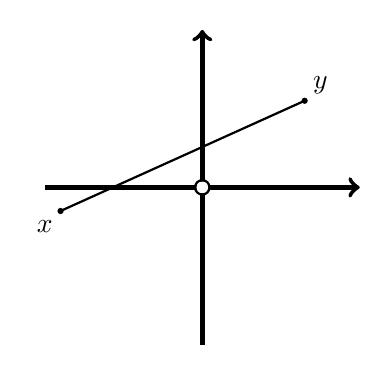
\begin{tikzpicture}[scale = 1]
            \draw[->,ultra thick] (-2,0)--(2,0) {};
            \draw[->,ultra thick] (0,-2)--(0,2) {};
            \node[circle, fill, white, inner sep=1.5pt] at (0, 0) {};
            \draw[black, thick] (0,0) circle[radius=2.6pt];
            \node[label] at (1.5, 1.3) {$y$};
            \node[circle, fill, black, inner sep=0.8pt] at (1.3, 1.1) {};
            \node[label] at (-2, -0.5) {$x$};
            \node[circle, fill, black, inner sep=0.8pt] at (-1.8, -0.3) {};
            \draw[-,thick](1.3, 1.1) -- (-1.8,-0.3);
        \end{tikzpicture}\\
        Case $1$
        \end{center}
    \end{minipage}\begin{minipage}{0.5\textwidth}
        \begin{center}
        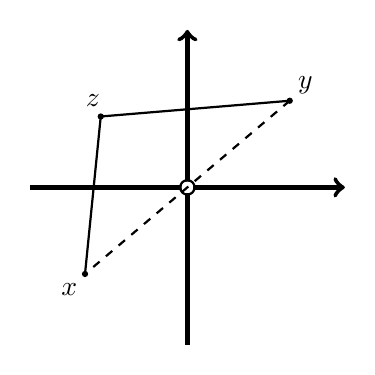
\begin{tikzpicture}[scale = 1]
            \draw[->,ultra thick] (-2,0)--(2,0) {};
            \draw[->,ultra thick] (0,-2)--(0,2) {};
            \node[circle, fill, white, inner sep=1.5pt] at (0, 0) {};
            \draw[black, thick] (0,0) circle[radius=2.6pt];
            \node[label] at (1.5, 1.3) {$y$};
            \node[circle, fill, black, inner sep=0.8pt] at (1.3, 1.1) {};
            \node[label] at (-1.5, -1.3) {$x$};
            \node[circle, fill, black, inner sep=0.8pt] at (-1.3, -1.1) {};
            \node[label] at (-1.2, 1.1) {$z$};
            \node[circle, fill, black, inner sep=0.8pt] at (-1.1, 0.9) {};
            \draw[dashed,thick](1.3, 1.1) -- (-1.3,-1.1);
            \draw[thick](-1.3, -1.1) -- (-1.1, 0.9);
            \draw[thick](-1.1, 0.9) -- (1.3, 1.1);
        \end{tikzpicture}\\
        Case $2$
        \end{center}
    \end{minipage}
    Explicitly in case $2$, $z \in X$ is a point not on the line though $x$ and $y$ and $f$ is the path
    $$f = \begin{cases} x(1-t) + zt &\text{ if }\,\,\, t \in [0,1]\\
    z(2-t) + (t-1)y & \text{ if }\,\,\,
t \in [1, 2]
    \end{cases}$$
    Moral: if $n = 1$, then $X$ is not path connected. Indeed, $X$ has two path components, namely $(-\infty, 0)$ and $(0, \infty)$, so that any path in $X$ has image contained in $(-\infty, 0)$ or $(0, \infty)$. In particular, there is no path from $1$ to $-1$ in $X$.
\item[3).] For each $n \geqslant 1$, the $n$-sphere
    $$S^n = \left\{x \in \R^n \mid ||x||^2 = 1\right\}$$
is (path) connected. Indeed, let $x, y \in S^n$. The great arc from $x$ to $y$ is a path from $x$ to $y$.
\item[4).] Let 
    $$X = \left\{\left(x, \sin{\dfrac{1}{x}}\right)\Big| 0 < x \leqslant 1\right\} \subset \R^2$$
    Then $X$ is (path) connected, being the image of the (path) connected space $(0, 1]$ under the continuous map $\sin{\dfrac{1}{x}}$. The closure $\overline{X}$ is called the {\bf Topologist's Sine Curv e}.
    $$\overline{X} = X \cup \left\{(0, y) \mid -1 \leqslant y \leqslant 1\right\}.$$
    \begin{center}
    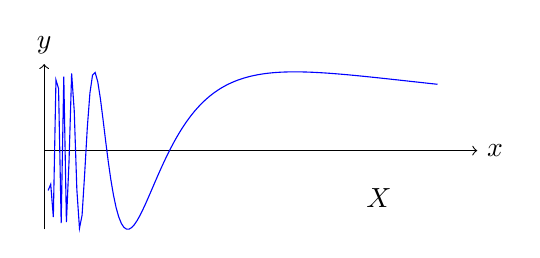
\begin{tikzpicture}[x=5cm]
        \draw[->] (0,0) -- (1.1,0) node[right] {$x$};
        \draw[->] (0,-1) -- (0,1.1) node[above] {$y$};
        \draw[blue,domain=0.01:1,samples=150] plot (\x, {sin((1/\x)r)});
        \node[label] at (0.85, -0.6) {$X$};
        \end{tikzpicture}
        \hspace{0.2cm}
    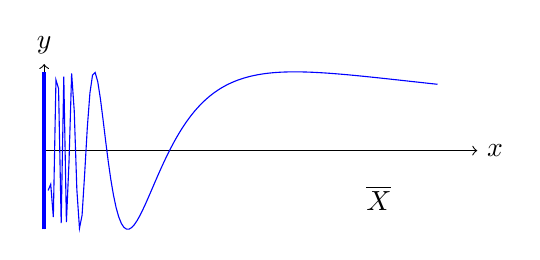
\begin{tikzpicture}[x=5cm]
        \draw[->] (0,0) -- (1.1,0) node[right] {$x$};
        \draw[->] (0,-1) -- (0,1.1) node[above] {$y$};
        \draw[blue,domain=0.01:1,samples=150] plot (\x, {sin((1/\x)r)});
        \draw[ultra thick, blue] (0, -1) -- (0, 1) {};
        \node[label] at (0.85, -0.6) {$\overline{X}$};
        \end{tikzpicture}\\
    (Note: Change the sample size in the \LaTeX\, source to make the graph smoother.)
    \end{center}
    The closure is connected. However, $\overline{X}$ is {\bf not} path connected. Say $f:[0, 1] \longrightarrow \overline{X}$ is a continuous function with 
    $$f(0) = (0, 0), \,\,\,f(1) \in X$$
    Since $A = \{0\} \times [-1, 1] \subset \overline{X}$ is closed, so too is $f^{-1}(A) \subset [0, 1]$. So, $f^{-1}(A)$ has a maximal element, say, $a$. Then $f(a)\in A$ while $f(t) \in X$ if $t > a$.\\
    Write $f$ in components: $f(t) = \left(x(t), y(t)\right)$. Then $x(a) = 0$ and $x(t) > 0$ and $y(t) = \sin{\dfrac{1}{x(t)}}$ if $t > a$. By the condition $x(t) > 0$ if $t > a$, for each $n \geqslant 1$, there exists a 
    $$0 < u < x\left(a + \dfrac{1}{n}\right)$$
    such that $\sin{\dfrac{1}{u}} = (-1)^n$. By the Intermediate Value Theorem, there exists a $0 < t_n < \dfrac{1}{n}$ such that $x(t_n) = u$. Then $\left\{t_n\right\}_n$ converges to $0$ but $y(t) = (-1)^n$ does not converge, a contradiction.
\end{enumerate}
\end{customexa}


\begin{customexa}{d.5.5} Here are some examples for \hypertarget{ex.d.5.5}{\hyperlink{Definition_5.5}{Definition $5.5$}}.
\begin{enumerate}
    \item[1).] Let $X$ be a finite topological space. Then $X$ is compact.\\
                Let $\left\{U_i\right\}_{i \in I}$ be an arbitrary open cover. So, 
                $$X = \underaccent{i \in I}{\bigcup} U_i $$
                For each $x \in X$, choose $i(x) \in I$ such that 
                $$x \in U_{i(x)}$$
                Then 
                $$X = \underaccent{x \in X}{\bigcup} U_{i(x)}$$
                So, $\left\{U_{i(x)}\right\}_{x\in X}$ is a finite subcover.
    \item[2).] Let $X =\left\{\dfrac{1}{n} \mid n \geqslant 1,\, n \in \mathbb{Z}\right\} \subset \R$. To prove it's not compact, we need to provide an open cover with no finite cover.\\
                For each $n \geqslant 1$, let $\widetilde{U}_n \subset \R$ be the open interval 
                $$\widetilde{U}_n = \left(\dfrac{1}{n} - \widetilde{\epsilon}_n, \dfrac{1}{n} + \epsilon_n\right)$$
    \item[3).] Let $X =\overline{\left\{\dfrac{1}{n} \mid n \geqslant 1\right\}} = \{0\} \cup \left\{\dfrac{1}{n} \mid n \geqslant 1\right\}$. Let $\left\{U_i\right\}_{i \in I}$ be an open cover of $X$. Let $i_0 \in I$ such that $0 \in U_{i_0}$. Since $U_{i_0}$ is open, there exists an $N > 0$ such that $\dfrac{1}{n} \in U_{i_0}$ whenever $n \geqslant N$. For $1, \dots , N-1$, choose open sets $U_{i_1}, \dots, U_{i_{N-1}}$ such that $\dfrac{1}{n} \in U_{i_n}$ for $n = 1, \dots, N -1$. Then 
    $$\left\{U_{i_0}, U_{i_1}, \dots, U_{i_{N-1}}\right\}$$
    is a finite subcover. So, $X$ is compact.
    \item[4).] The open interval $(0, 1)$ is not compact. Indeed, consider the open cover $\left\{\left(\dfrac{1}{n}, \dfrac{1}{n +2}\right)\mid n \geqslant 1\right\}$. \\
    Let $I \subset \mathbb{Z}_{> 0}$ be a finite subset. Let $N > 0$ such that $N > i$ for all $i \in I$. Then $\dfrac{1}{N + 4} \notin \underaccent{i \in I}{\bigcup} U_i$. So, this open cover has no finite subcover.
\end{enumerate}
\end{customexa}

\begin{customexa}{t.5.14} Here is an example for \hypertarget{ex.t.5.14}{\hyperlink{Theorem_5.14}{Theorem $5.14$}}.\\
Recall the diagram:
\begin{center}
    \begin{tikzpicture}[scale = 1.5]
    \node[label] at (0,1) {$[0,1]$};
    \node[label] at (1.6,-0.8) {$S^1$};
    \node[label] at (-2.3,-1) {$[0, 1]/_{\sim}$};
    \draw[-stealth](0.2,0.8) -- (1.4,-0.6);
    \draw[-stealth](-0.2,0.8) -- (-1.8,-0.8);
    \draw[-stealth](-1.8,-1) -- (1.4,-0.8);
    \node[label] at (2, 0.4) {$f(x) = \left(\cos{2 \pi x}, \sin{2 \pi x}\right)$};
    \node[label] at (-1,0.3) {$q$};
    \node[label] at (-0.3,-1.2) {$\widetilde{f}$};
    \end{tikzpicture}
\end{center}
The space $[0,1]$ is compact (Theorem $5.12$), and hence so too is $[0, 1]/_{\sim}$ (Theorem $5.11$). The space $S^1$ is Hausdorff, being a subspace of the Hausdorff space $\R^2$ (Theorem 2.20). The function $\widetilde{f}$ is a continuous bijection and so is a homeomorphism by Theorem $5.14$.

\end{customexa}

\newpage
\phantomsection
\section*{6. Surfaces}
\addcontentsline{toc}{section}{6. Surfaces}

\begin{customexa}{d.6.1} Here are some examples for \hypertarget{ex.d.6.1}{\hyperlink{Definition_6.1}{Definition $6.1$}}.
\begin{enumerate}
    \item[1).] $\R$ is second countable:
                $$\mathcal{B}' = \left\{B_{\epsilon}(x) \mid x\in \mathbb{Q}, \epsilon \in \mathbb{Q} \cap (0, \infty)\right\}$$
    \item[2).] If $X, Y$ are second countable, then $X \times Y$ is second countable.
    \item[3).] If $X$ is second countable, $A \subset Y$ is second countable.
    \item[4).] $\R \times \R_{dis}$ is not second countable. (Note: the discrete topology by itself is not second countable.)
\end{enumerate}
\emph{Comment:} $1) \sim 3)$ implies that any subspace of $\R^n$ is second countable.
\end{customexa}

\begin{customexa}{d.6.2} Here are some examples for \hypertarget{ex.d.6.2}{\hyperlink{Definition_6.2}{Definition $6.2$}}.
\begin{enumerate}
    \item[1).] The sphere $S^n$ is an $n$-manifold:
        \begin{enumerate}
            \item[i).] It is a subspace of $\R^{n + 1}$, hence Hausdorff
            \item[ii).] It is a subspace of $\R^{n + 1}$, hence second countable
            \item[iii).] The locally Euclidean condition can be seen by intersection with open hemispheres:
        \end{enumerate}
\end{enumerate}
\end{customexa}


\newpage
\phantomsection
\addcontentsline{toc}{chapter}{Appendix 3. Iconic Questions}

\phantomsection
\section*{1. Sets and Continuity}
\addcontentsline{toc}{section}{1. Sets and Continuity}

\begin{cusques}{1.1}[Finite and Infinite Sets] The following are checking basic understandings of set theory and the foundations of the axioms of topology.
\begin{enumerate}
    \item[(a).] A finite subset of $\R^n$ is closed.
    \begin{proof}
        This is true. Consider $A = \left\{x_1, \dots, x_n\right\} \subset \R^n$ a finite subset. Then we can write 
            $$A = \left(\bigcup_{i=1}^{n}\left(\R^n \setminus \left\{x_i\right\}\right)\right)^c$$
        As the sets $\R^n\setminus\left\{x_i\right\}$ are open, so is their intersection. Thus $A$ is closed, being the complement of an open set.
    \end{proof}
    \item[(b).] If $\tau$ and $\sigma$ are topologies on a set $X$, then so too are
    $$\tau \cap \sigma := \left\{U \mid U \in \tau \text{ and } Y \in \sigma\right\} \,\,\,\,\text{ and }\,\,\,\, \tau \cup \sigma := \left\{U \mid U \in \tau \text{ or } Y \in \sigma\right\}$$
    \begin{proof}
        This is false. The intersection of two topologies is again a topology using the definition of a topology. However the union of two topologies is not necessarily a topology again. Consider $A = \left\{1,\, 2,\, 3\right\}$. Then $\tau = \left\{\varnothing,\, \{1\},\, \{1, 2\},\, A \right\}$ is a topology on $A$ and $\sigma = \left\{\varnothing,\, \{3\},\, \{2, 3\},\, A \right\}$ is as well, but in their union the finite intersection $\left\{1,\, 2\right\} \cap \left\{2,\, 3\right\} = \left\{2\right\}$ is not contained.
    \end{proof}
    \item[(c).] Let $\left\{A_i\right\}_{i \in I}$ be an arbitrary collection of closed subsets of $\R^n$. Then $\underaccent{i \in I}{\bigcup}A_i \subset \R^n$ is closed.
    \begin{proof}
        This is false. It suffices to produce a counterexample for $n =1$. For each positive integer $i$, define a closed subset of $\R$ by 
            $$A_i = \left[0, 1 - \dfrac{1}{i}\right]$$
        The union $\bigcup\limits_{i=1}^{\infty} A_i = [0, 1)$ is not closed: every open interval centered at $1$ intersects $A$.
    \end{proof}
\end{enumerate}
\end{cusques}


\begin{cusques}{1.2}[Proving Topologies] The following are checking the understanding the axioms of topology.
\begin{enumerate}
    \item[(a).] Let 
        $$\tau = \left\{U \subset \R \mid \text{ for all } u \in U, \text{ there exists } a < b \text{ such that } u \in [a, b) \subset U\right\}.$$
        Prove that $\tau$ is a topology on $\R$.
        \begin{proof} We need to verify the three axioms for a topology:
            \begin{enumerate}
                \item[i.] Any real number lies in an interval of the form $[a, b)$, thus it is clear that $\varnothing,\, \R$ lie in $\tau$.
                \item[ii.] Let $\left\{U_i\right\}_{i \in I}$ be an arbitrary collection of elements of $\tau$ and set $U = \underaccent{i \in I}{\bigcup}U_i$. Let $u \in U$. Then $u \in U_i$ for some $i \in I$. Since $U_i$ is open, there exists an $a \in \R$ such that $u \in [a, b) \subset U_i$. But then $u \in [a, b) \subset U$, so that $U \in \tau$.
                \item[iii.] Let $\left\{U_i\right\}_{i \in I}$ be an finite collection of elements of $\tau$ and set $U = \underaccent{i \in I}{\bigcap} U_i$. Let $u \in U$. Then $u \in U_i$ for each $i \in I$. Since $U_i$ is open, there exists $a_i, b_i \in \R$ such that $u \in [a_i,\, b_i)$. Let $a = \text{max}\left\{a_i\mid i \in I\right\}$ and $b = \text{min}\left\{b_i \mid i \in I\right\}$. Since $I$ is finite, $a$ and $b$ are well-defined real numbers, and they still fulfill $a<b$. Then $u \in [a,\, b)$ and, since $[a,\, b) \subset [a_i,\, b_i) \subset U_i$ for all $i \in I$, we have $u \in [a,\, b) \subset U$. Hence, $U\in \tau$.
            \end{enumerate}
        \end{proof}
    \item[(b).] Let 
\end{enumerate}
\end{cusques}

\newpage
\phantomsection
\section*{2. Topological Spaces}
\addcontentsline{toc}{section}{2. Topological Spaces}

\begin{cusques}{2.1}[Basis] The following are checking basic understandings of basis of a topology.
\begin{enumerate}
    \item[(a).] What is a basis for a topology on $\R$?
    \begin{proof}
    \end{proof}
\end{enumerate}
\end{cusques}

\begin{cusques}{2.2}[Subspace Topology] The following are checking basic understandings of subspace construction of topological spaces.
\begin{enumerate}
    \item[(a).] 
    \begin{proof}
    \end{proof}
\end{enumerate}
\end{cusques}

\begin{cusques}{2.3}[Product Topology] The following are checking basic understandings of product construction of topological spaces.
\begin{enumerate}
    \item[(a).] 
    \begin{proof}
    \end{proof}
\end{enumerate}
\end{cusques}

\phantomsection
\addcontentsline{toc}{subsection}{Hausdorff Spaces}

\begin{cusques}{2.4}[Hausdorff] Prove that a topological space $X$ is Hausdorff if and only if the diagonal 
$$\Delta = \left\{\left(x, x\right) \mid x \in X\right\}$$
is closed in $X \times X$
    \begin{proof}
    \end{proof}
\end{cusques}

\begin{cusques}{2.?}[Interiors and Closures] The following are checking the understandings of interiors and closures
\begin{enumerate}
    \item[(a).] $\text{Int} \left(\mathbb{Q}\right) = \varnothing, \,\,\, \overline{\mathbb{Q}} = \R$
    \begin{proof}
    For the interior, since it's the union of all open sets contained in $\mathbb{Q}$, then $\forall q \in \mathbb{Q}, \, \forall \epsilon > 0, \, B_{\epsilon}q = \left\{x \in \R \mid |x - q| < \epsilon\right\}$ contains irrational numbers that are not in $\mathbb{Q}$. So the only open interval we can have is the $\varnothing$, hence, $\text{Int} \left(\mathbb{Q}\right) = \varnothing$. Note, if the whole set is $\mathbb{Q}$, then $\text{Int} \left(\mathbb{Q}\right) = \mathbb{Q}$.\\
    For the closure, since it's the intersection of all closed sets of $\R$ which contain $\mathbb{Q}$, we can assume $\mathbb{Q} \subset C \subset \R$, for some closed set $C$. Then, $\R \setminus C$ must be open since the complement of a closed set is open. However, every single open interval of $\R$ has to include some rational numbers, and $\mathbb{Q}$ is out of the picture because $\mathbb{Q} \subset C$. Therefore, $\R \setminus C$ can only be $\varnothing$, then $C = \R$.
    \end{proof}
    \item[(b).] Find the closure, interior and boundary of each of the following subsets of $\R^2$
        \begin{enumerate}
            \item[i)] 
        \end{enumerate}
\end{enumerate}
\end{cusques}



\newpage
\phantomsection
\section*{3. Continuous Functions}
\addcontentsline{toc}{section}{3. Continuous Function}

\newpage
\phantomsection
\section*{4. More Topological Spaces}
\addcontentsline{toc}{section}{4. More Topological Spaces}

\newpage
\phantomsection
\section*{5. Connectedness and Compactness}
\addcontentsline{toc}{section}{5. Connectedness and Compactness}

\newpage
\phantomsection
\section*{6. Surfaces}
\addcontentsline{toc}{section}{6. Surfaces}
\end{document}